
\documentclass[12pt]{amsart}   % LaTeX with AMS style; 12 point for old eyes

\usepackage{amssymb,amsfonts}   % For better support of math
\usepackage{graphicx}	        % Enable for eps and pdf figures, if they occur
\usepackage{hyperref}           % Enable embedded hyperlinks.
\usepackage[bottom]{footmisc}
\usepackage{listings}
\usepackage{float}
\usepackage[most]{tcolorbox}
\usepackage{inconsolata}

% Commands to force sequential numbering:

\newtheorem{theorem}{Theorem}[section]
\newtheorem{proposition}[theorem]{Proposition}
\newtheorem{lemma}[theorem]{Lemma}
\newtheorem{definition}[theorem]{Definition}
\newtheorem{examples}[theorem]{Examples}
\newtheorem{remarks}[theorem]{Remarks}
\newtheorem{corollary}[theorem]{Corollary}
\newtheorem{remark}[theorem]{Remark}
\newtheorem{example}[theorem]{Example}
\newtheorem{conjecture}[theorem]{Conjecture}

\begin{document}

\title[CSE380 Project 1]{CSE380 Tools and Techniques for Computational Science Project 1  \\[Modeling document]} 
% the first [...] gives a brief version of the title, which is long!
 
\author{Mohammad Afzal Shadab}\email{mashadab@utexas.edu}
\date{\today}              % or an actual date


\newcommand{\C}{\mathbb C} % blackboard bold , for ``complex,'' etc
\newcommand{\R}{\mathbb R} 
\newcommand{\Z}{\mathbb Z}
\newcommand{\Q}{\mathbb Q}
\newcommand{\N}{\mathbb N}

\begin{abstract}
This is a \textit{modeling document} for the application to solve the steady-state heat equation in one- and two-dimensions. The document highlights the governing equations, boundary conditions, numerical approximations, and high-level pseudocode implemented in the solver. Then we have described the files used in the software including C++, Python, shell scripts and text files. We have also outlined the procedures for building and running the codes and its testing. Next, we show the results of testing mainly verification, regression and runtime performance testing. We have used these libraries: {\tt{GRVY}} for time-keeping and debugging, {\tt{MASA}} for manufactured solutions, {\tt{bats}} for designing regression tests. Finally, we have shown some results and compared them with analytical results.
\end{abstract}

\maketitle

\section{Governing equations and boundary conditions\label{sec:goveqn}}
The steady-state heat equation with a constant coefficient in two dimensions is given by:
\begin{equation} \label{eq:1}
    \boxed{-k \nabla^2T(x,y) = q(x,y) \quad \forall \Omega\in[0,L]\times[0,H]}
\end{equation}
where $k$ is the thermal conductivity (W/K), $T(x,y)$ is the material temperature (K), $q(x,y)$ is a heat source term (W/m$^2$) and $\Omega \subset \mathbb{R}^2$ is the domain. This is Poisson equation which is a type of elliptic partial differential equations. This linear boundary value problem is subjected to either \textit{Dirichlet boundary conditions} ($T$ specified) following \textit{maximum principle} or combinations of \textit{Neumann} ($\nabla T$ specified), \textit{Dirichlet} and \textit{Robin boundary conditions}. To begin with, let's specify Dirichlet boundary conditions:
\begin{eqnarray}
T(0,y) &=& T_{analytical}(0,y) \nonumber\\
T(L,y) &=& T_{analytical}(L,y)\\
T(x,0) &=& T_{analytical}(x,0)\nonumber\\
T(x,H) &=& T_{analytical}(x,H)\nonumber
\end{eqnarray}
where $T_{analytical}$ is evaluated using MASA.
\section{Assumptions \label{sec:assumptions}}
We'll start with the assumptions for the derivation of equation \ref{eq:1} from the law of conservation of energy in Eulerian framework \ref{eq:3} \cite{oden2011introduction}:
    \begin{equation} \label{eq:3}
        \frac{ \partial }{ \partial t }{(\rho e) + \nabla \cdot(\rho e \textbf{u}) = \textbf{T}:\textbf{D} -\nabla \cdot \textbf{q} + r}
    \end{equation}
where $e$ is internal energy per unit mass, $\textbf{T}:\textbf{D}$ is the strain heating, $\textbf{q}$ is the heat flux and $r$ is the volumetric source / sink. 
\begin{itemize}
\item Continuum assumption
    \item Steady-state ($\partial(.) / \partial t = 0$)
    \item No advection $\textbf{u}=\textbf{0}$
    \item No source/sink term $r=0$
    \item Validity of \textit{Fourier's law of heat conduction}, i.e., $\textbf{q} =-k \nabla T$
    \item No strain heating, i.e., $\textbf{T : D}=0$, where $\textbf{T}$ is the stress tensor and $\textbf{D}$ is the deformation tensor
    \item Constant coefficient of thermal conductivity $k$
\end{itemize}

Moving towards the assumptions to make the numerical implementation easier:
\begin{itemize}
    \item Square domain $L\equiv H$
    \item Uniform grid, i.e. $N_x=N_y=N$, where $N_x$ and $N_y$ are the cells in x and y directions respectively. So, $\Delta x = \Delta y = h$
    \item The Dirichlet boundary conditions are implemented in form of constant temperatures in the ghost cells adjacent to a corresponding boundary, i.e., $T_{0,1}=T_{analytical}(x_0,y_1)$
\end{itemize}

\section{Nomenclature}
For 1D, the mesh numbering is simple and straight forward, as shown in figure \ref{fig:1}. The scheme is cell based, where cell centers $(x_c,y_c)$ are referred. For 2D mesh, the situation is slightly sophisticated as two indices $(i,j)$ come to picture correspondingly in x and y directions illustrated in figure \ref{fig:2}. So, using a new numbering system for converting $(i,j)$ into one index $l$ which first spans x direction cells then marches in y direction.

\begin{figure}[b!]
\hspace{1cm}
    \centering
    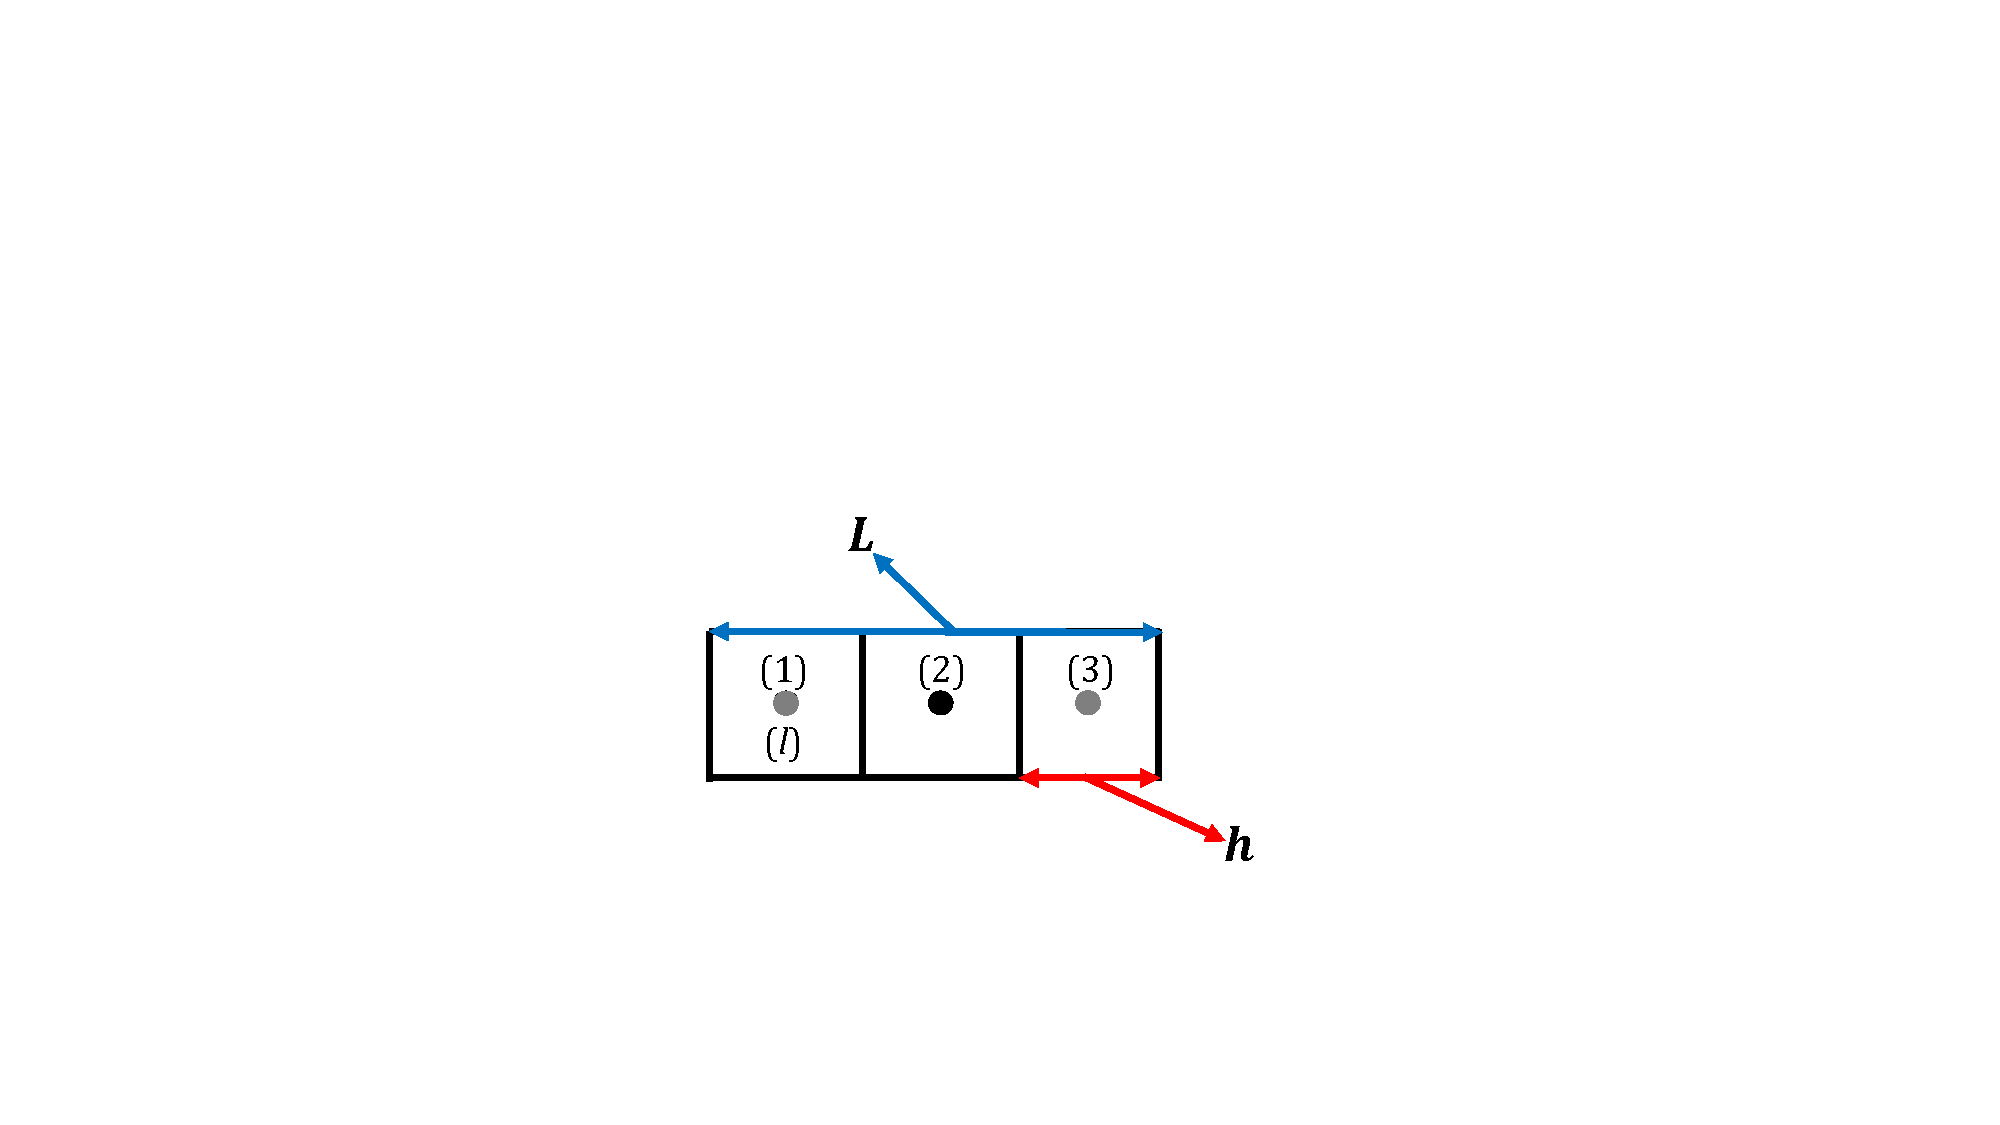
\includegraphics[width=0.5\linewidth]{HW4 figures-4.pdf}
    \caption{1D mesh with 3 cells, grey dots which represent boundary cell centers, and $l$ indexing}
    \label{fig:1}
\end{figure}


\begin{eqnarray}
l &=& i+(j-1)N_x, & \text{$l$}\in\{1,2,...,N_x*N_y\} \nonumber\\
l\%N_x &=& i & \text{(Remainder)}  \\
l/N_x &=& j-1 &\text{(Integer division)}  \nonumber 
\end{eqnarray}

\begin{figure}
    \centering
    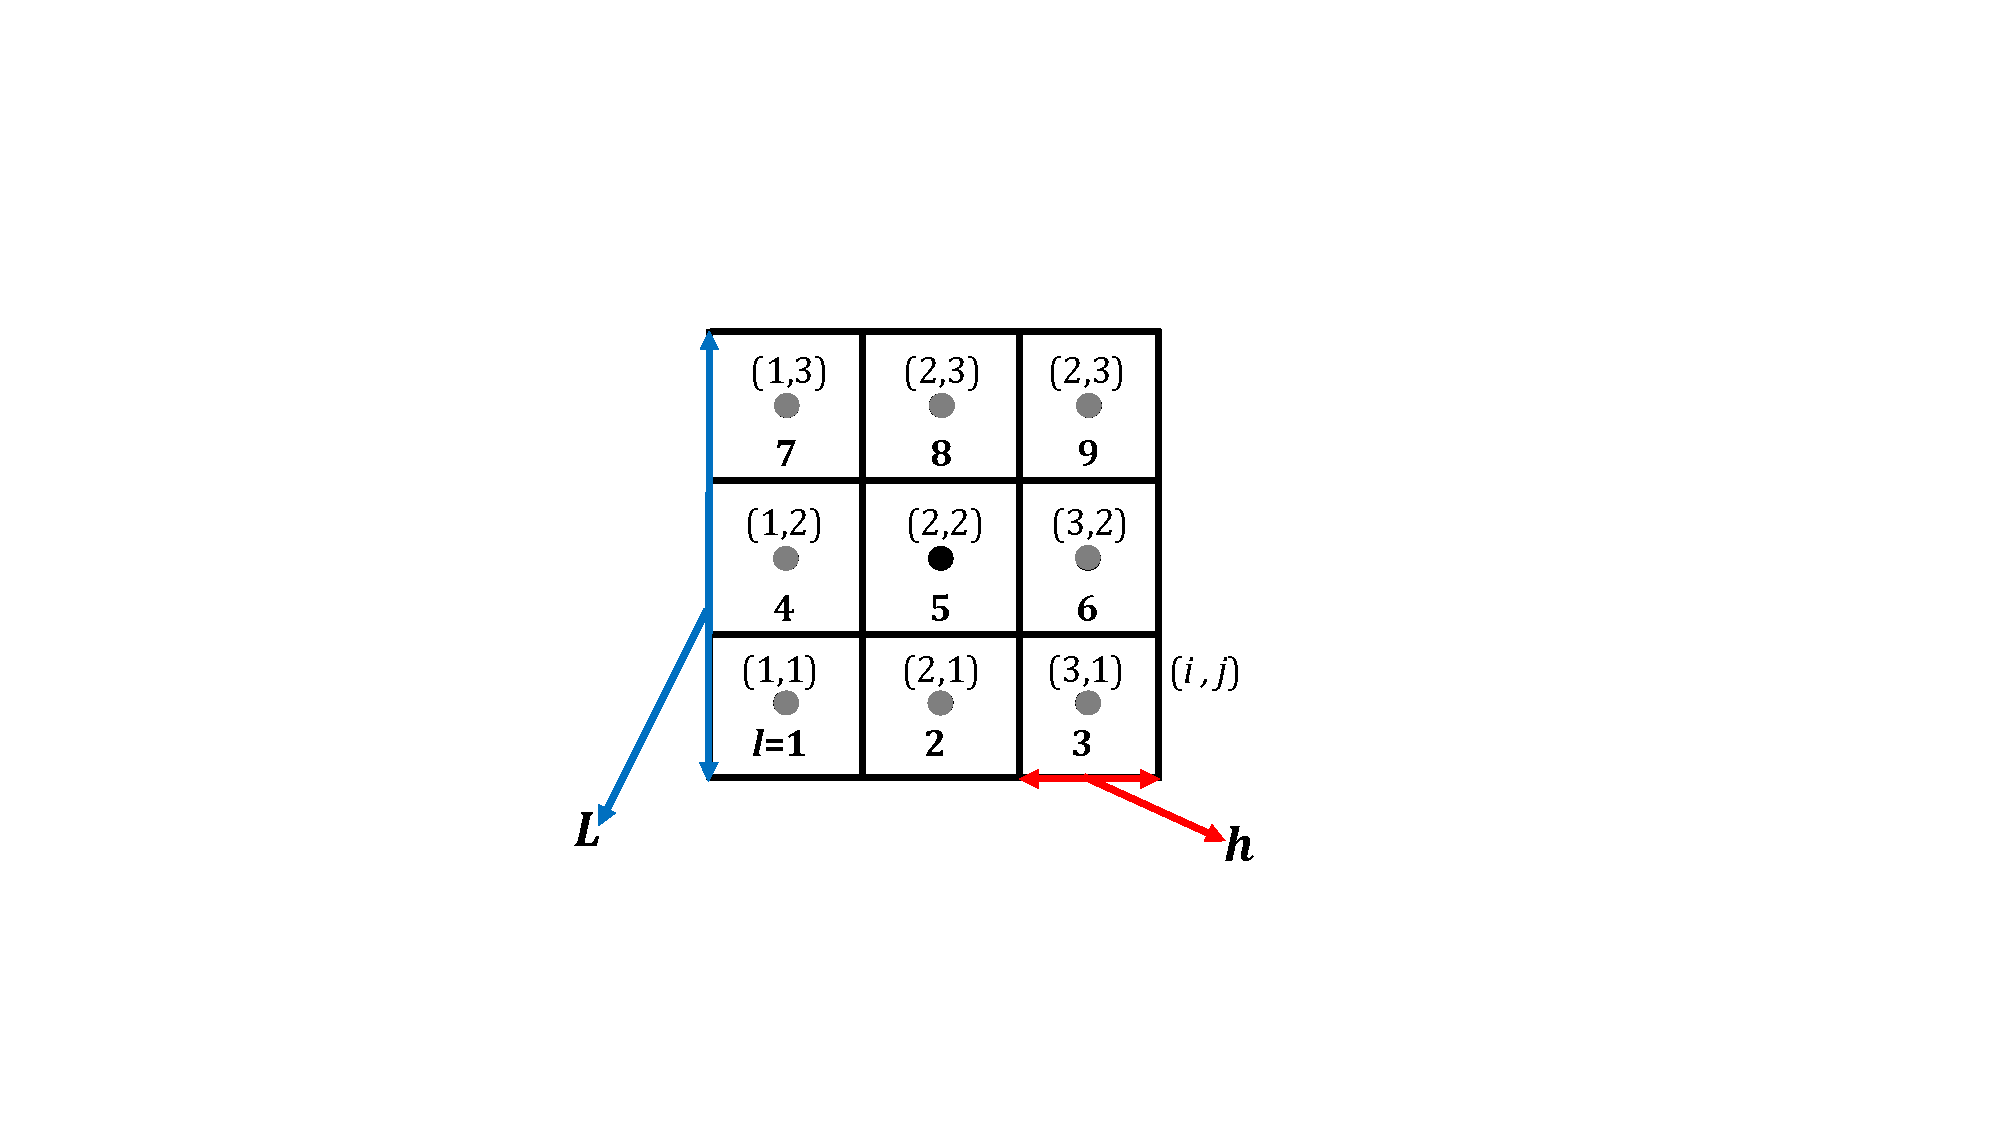
\includegraphics[width=0.75\linewidth]{HW4 figures-3.pdf}
    \caption{2D $3\times3$ uniform mesh with boundary cells centers shown in grey, $(i,j)$ indexing, and universal $l$ indexing}
    \label{fig:2}
\end{figure}
The value at the centers of boundary cells are evaluated using MASA.

\section{Numerical Methods}
Finite difference approximation has been implemented considering the ease of implementation when compared with other discretization methods such as finite volumes, finite element, etc \cite{quarteroni2010numerical}. Rewriting equation \ref{eq:1} in expanded form for 1D
\begin{equation} \label{eq:5}
    -k \frac{\partial^2 T(x) }{\partial x^2} = q(x)
\end{equation}
and for 2D
\begin{equation}\label{eq:6new}
    -k \bigg(\frac{\partial^2 T(x,y) }{\partial x^2}+\frac{\partial^2 T(x,y) }{\partial y^2} \bigg) = q(x,y)
\end{equation}

\subsection{Second order finite difference approximation}
Using the Taylor's expansion, the second order central difference approximation for second order derivative in x direction can be written
\begin{equation}\label{eq:6}
 \frac{ \partial^2 T}{\partial x^2}=\frac{T_{i+1} -2T_{i} + T_{i-1}}{\Delta x^2}+\mathcal{O}(h^2)  
\end{equation}
where subscript $i$ is the cell centered value of cell $i$.
\subsubsection{1D} Equation \ref{eq:6} can be substituted into equation \ref{eq:5}, to give
\begin{equation}
-k \Bigg(\frac{T_{i+1} -2T_{i,j} + T_{i-1}}{\Delta x^2} \Bigg)+\mathcal{O}(h^2) = q_i
\end{equation}
Inserting $\lambda = -k/\Delta x^2$ and dividing by $\lambda$, we get
\begin{equation}
{T_{i+1} -2T_{i} + T_{i-1}} +\mathcal{O}(h^4) = q_i/\lambda
\end{equation}
Neglecting the truncation error $\mathcal{O}(h^4)$ and writing in matrix form for a 3 cell grid shown in figure \ref{fig:1} after implementing the boundary conditions, we get
\begin{equation}
 \begin{pmatrix}
1 &  &  \\
1 & -2 & 1 \\
 &  & 1 \\
\end{pmatrix} \begin{bmatrix}
T_{1}\\
T_{2}\\
T_{3}\\
\end{bmatrix} =
\begin{bmatrix}
T_{1,MASA}\\
{q_{2}}/\lambda\\
{T_{3,MASA}}\\
\end{bmatrix} \Rightarrow \textbf{AT=q}
\end{equation}

For a $N$-cell grid, the matrix equation takes the following form, 
\begin{equation}
\textbf{A}=\begin{pmatrix}
1 &  & & &&\\
1 & -2 & 1 && & \\
& 1 & -2 & 1 && \\
&  & \ddots & \ddots & \ddots& \\
&   && 1 &-2 &1\\
&   & & & &1\\
\end{pmatrix}, \textbf{T}=\begin{bmatrix}
T_{1}\\
{T_{2}}\\
\vdots\\
{T_{N-1}}\\
{T_{N}}\\
\end{bmatrix}, \textbf{q}=\begin{bmatrix}
T_{1,MASA}\\
{q_{2}}/\lambda\\
\vdots\\
{q_{N-1}}/\lambda\\
T_{N,MASA}\\
\end{bmatrix}
\end{equation}
So, the resulting matrix \textbf{A} is tridiagonal (\textcolor{red}{3 diagonals}).
\begin{equation}
\textbf{A}=\begin{pmatrix}
\times &  & & &&\\
\times & \times & \times && & \\
& \times & \times & \times && \\
&  & \ddots & \ddots & \ddots& \\
&   && \times & \times &\times\\
&   & & &  &\times\\
\end{pmatrix}\end{equation}


\subsubsection{2D}
We can write
\begin{equation}
    -k \Bigg(\frac{T_{i+1,j} -2T_{i,j} + T_{i-1,j}}{\Delta x^2}+\frac{T_{i,j+1} -2T_{i,j} + T_{i,j-1}}{\Delta y^2} \Bigg)+\mathcal{O}(h^2) = q_{i,j}
\end{equation}
where $i$ and $j$ are the positions of cell center in x and y directions. Using $\Delta x = \Delta y = h$ from assumptions and $-k/h^2 = \lambda$ we get
\begin{equation}
     T_{i+1,j} + T_{i-1,j}+T_{i,j+1} + T_{i,j-1} -4T_{i,j} +\mathcal{O}(h^4) = q_{i,j} / \lambda
\end{equation}

\begin{equation}
     T_{k,k+1} + T_{k,k-1}+T_{k,k+N_x} + T_{k,k-N_x} -4T_{k,k} +\mathcal{O}(h^4) = q_{k} / \lambda
\end{equation}
Implementing boundary conditions, for a $5\times5$ uniform grid, the repeating interior block of $\mathbf{A}$ is given by,
                    \begin{align*}
                    \mathbf{A}_{rep} = \left[\begin{matrix}
                    &&1\\ 1&\hdots&1&-4&1&\hdots&1\\
                     &1&\hdots&1&-4&1&\hdots&1\\
                     &&1&\hdots&1&-4&1&\hdots&1\\
                    &&&&&&1\\
                    \end{matrix}\right]
                \end{align*}
The rows corresponding to boundary entries only have a diagonal with value 1. 
\begin{align*}
                \mathbf{A} &= \left[\begin{smallmatrix} 
                \times\\
                & \times\\
                && \times\\
                &&& \times\\
                &&&& \times\\
                &&&&& \times\\
                 \times &&&&&\times& \times &\times&&&&& \times\\
                & \times &&&&&\times& \times &\times&&&&& \times\\
                && \times &&&&&\times& \times &\times&&&&& \times\\
                &&&&&&&&& \times\\
                &&&&&&&&&& \times\\
                &&&&& \times &&&&&\times& \times &\times&&&&& \times\\
                &&&&&& \times &&&&&\times& \times &\times&&&&& \times\\
                &&&&&&& \times &&&&&\times& \times &\times&&&&& \times\\
                &&&&&&&&&&&&&& \times\\
                &&&&&&&&&&&&&&& \times\\
                &&&&&&&&&& \times &&&&&\times& \times &\times&&&&& \times\\
                &&&&&&&&&&& \times &&&&&\times& \times &\times&&&&& \times\\
                &&&&&&&&&&&& \times &&&&&\times& \times &\times&&&&& \times\\
                &&&&&&&&&&&&&&&&&&& \times\\
                &&&&&&&&&&&&&&&&&&&& \times\\
                &&&&&&&&&&&&&&&&&&&&& \times\\
                &&&&&&&&&&&&&&&&&&&&&& \times\\
                &&&&&&&&&&&&&&&&&&&&&&& \times\\
                &&&&&&&&&&&&&&&&&&&&&&&& \d\\
                \end{smallmatrix}\right]
            \end{align*}
So, we have 
\begin{equation}
    \Rightarrow \textbf{AT}&=&\textbf{q}
\end{equation}
where
\begin{align*}
                    \mathbf{q} &= \left[T_{1,MASA},T_{2,MASA} \hdots,q_{N+1}/\lambda , \hdots,q_{N*N-N}/\lambda,\hdots, T_{MASA}(x_{N*N-1}),T_{N*N,MASA}\right]^T\\
                    \mathbf{T} &= [T_1 ,\hdots, T_{N*N}]^T
                \end{align*}

For a general matrix,
\begin{equation}
A = \begin{cases}
A_{l-N_x,l}= \begin{cases}
1 & l/N_x = 0 \\
0 & \text{else (bottom boundary)}
\end{cases}\\
A_{l-1,l}= \begin{cases}
1 & l\% N_x > 1  \\
0 & \text{else (left boundary)}
\end{cases} \\
A_{l,l}= \begin{cases}
-4 & \text{(interior)} \\
1 & \text{else (boundary)}
\end{cases} \\
A_{l+1,l}= \begin{cases}
1 & l\% N_x ~= 0 \\
0 & \text{else (right boundary)}
\end{cases} \\
A_{l-N_x,l}= \begin{cases}
1 & l/N_x = N_y-1 \\
0 & \text{else (top boundary)}
\end{cases}\\
\end{cases}
\end{equation}

\subsection{Fourth order finite difference approximation}
Using the Taylor's expansion, the fourth order central difference approximation for second order derivative in x direction can be written as:
\begin{equation}\label{eq:19}
 \frac{ \partial^2 T}{\partial x^2}=\frac{-T_{i+2}+16T_{i+1} -30T_{i} + 16T_{i-1} - T_{i-2}}{\Delta 12x^2}+\mathcal{O}(h^4)
\end{equation}
where subscript $i$ is the cell centered value of cell $i$.
\subsubsection{1D} Equation \ref{eq:19} can be substituted into equation \ref{eq:5}, to give
\begin{equation}
-k \Bigg(\frac{-T_{i+2}+16T_{i+1} -30T_{i} + 16T_{i-1} - T_{i-2}}{\Delta 12x^2} \Bigg)+\mathcal{O}(h^4) = q_i
\end{equation}
Inserting $\lambda = -k/\Delta x^2$ and dividing by $\lambda$, we get
\begin{equation}
{-T_{i+2}+16T_{i+1} -30T_{i} + 16T_{i-1} - T_{i-2}} +\mathcal{O}(h^6) = q_i/\lambda
\end{equation}
Neglecting the truncation error $\mathcal{O}(h^6)$ and writing in matrix form for an $N$ cell grid shown in figure \ref{fig:1} after implementing the boundary conditions, we get
\begin{equation}
\Rightarrow \textbf{AT=q}
\end{equation}
where 
                \begin{align*}
                    \mathbf{q} &= \left[T_{1,MASA} ,T_{2, MASA},q_{3}/\lambda \hdots,q_{N-1}/\lambda, T_{N-1,MASA},T_{N,MASA}\right]^T\\
                    \mathbf{T} &= [T(0) ,\hdots, T(N)]^T
                \end{align*}
                
                
                \begin{align*}
                    \mathbf{A} &= \begin{bmatrix} 
                    1\\
                    & 1 &   \\
                    -1 & 16 & -30 & 16 & -1  \\
                    &-1 & 16 & -30 & 16 & -1  \\
                    &&-1 & 16 & -30 & 16 & -1  \\
                    &&& \ddots&\ddots&\ddots&\ddots&\ddots\\
                    &&&& -1 & 16 & -30 & 16 & -1 \\
                    &&&&& -1 & 16 & -30 & 16 & -1\\
                    &&&&&&& & 1 &\\
                    &&&&&&&&& 1
                    \end{bmatrix}
                \end{align*}

So, the resulting matrix \textbf{A} is pentadiagonal (\textcolor{red}{5 diagonals})
\begin{align*}
                    \mathbf{A} &= \begin{bmatrix} 
                    \times\\
                     & \times &   \\
                    \times & \times & \times & \times & \times  \\
                    &\times & \times & \times & \times & \times  \\
                    && \times & \times & \times & \times & \times  \\
                    &&& \ddots & \ddots & \ddots & \ddots & \ddots  \\
                    &&&& \times & \times & \times & \times & \times \\
                    &&&&& \times & \times & \times & \times & \times\\
                    &&&&&&&  & \times & \\
                    &&&&&&&&& \times
                    \end{bmatrix}
                \end{align*}
                
\subsubsection{2D} Equation \ref{eq:19} can be substituted into equation \ref{eq:6}, to give
\begin{eqnarray}
-k \Bigg(\frac{-T_{i+2,j}+16T_{i+1,j} -30T_{i,j} + 16T_{i-1,j} - T_{i-2,j}}{\Delta 12x^2} &+& \nonumber \\ \frac{-T_{i,j+2}+16T_{i,j+1} -30T_{i,j} +
16T_{i,j-1} - T_{i,j-2}}{\Delta 12y^2} \Bigg) &+& \mathcal{O}(h^4) = q_{i,j} \nonumber\\
\end{eqnarray}
where $i$ and $j$ are the positions of cell center in x and y directions. Implementing, $\Delta x = \Delta y = h$ from assumptions and $-k/12h^2 = \lambda$
\begin{eqnarray}
-T_{i+2,j}+16T_{i+1,j}+16T_{i-1,j} -T_{i-2,j}-T_{i,j+2}+16T_{i,j+1}+16T_{i,j-1} - \nonumber \\ T_{i,j-2} -60T_{i,j}  +\mathcal{O}(h^6) = q_{i,j}/\lambda
\end{eqnarray}
Using $k$ indexing for blocks in same row, 
\begin{eqnarray}
-T_{k+2,k}+16T_{k+1,k}+16T_{k-1,k} -T_{k-2,k}-T_{k+2N_x,k}&+16T_{k+N_x,k}+ \nonumber \\ 16T_{k-N_x,k} - T_{k-2N_x,k}-60T_{k,k} &+\mathcal{O}(h^6) = q_{k}/\lambda
\end{eqnarray}
Neglecting the truncation error $\mathcal{O}(h^6)$ and writing in matrix form for $7 \times 7$ uniform grid after implementing the boundary conditions, we get
    \begin{align*}
                    \mathbf{AT} = \mathbf{q}
                \end{align*}
                where

            \begin{align*}
                \mathbf{A}_{rep} &= \left[\begin{smallmatrix} 
                &&&&&&&&&&& \ddots\\
                &&&&&&&&&&&& \times\\
                &&&&&&&&&&&&& \times\\
                &&&&&&&&&&&&&& \times\\
                &&&&&&&&&&&&&&& \times\\
                &&\times&&&&&&&\times&&&&&\times&\times&\times&\times&\times&&&&&\times&&&&&&&\times \\
                &&&\times&&&&&&&\times&&&&&\times&\times&\times&\times&\times&&&&&\times&&&&&&&\times \\
                &&&&\times&&&&&&&\times&&&&&\times&\times&\times&\times&\times&&&&&\times&&&&&&&\times \\
                &&&&&&&&&&&&&&&&&&&\times\\
                &&&&&&&&&&&&&&&&&&&&\times\\
                &&&&&&&&&&&&&&&&&&&&&\times\\
                &&&&&&&&&&&&&&&&&&&&&&\times\\
                &&&&&&&&&\times&&&&&&&\times&&&&&\times&\times&\times&\times&\times&&&&&\times&&&&&&&\times \\
                &&&&&&&&&&\times&&&&&&&\times&&&&&\times&\times&\times&\times&\times&&&&&\times&&&&&&&\times \\
                &&&&&&&&&&&\times&&&&&&&\times&&&&&\times&\times&\times&\times&\times&&&&&\times&&&&&&&\times \\
                &&&&&&&&&&&&&&&&&&&&&&&&&& \times\\
                &&&&&&&&&&&&&&&&&&&&&&&&&&& \times\\ 
                &&&&&&&&&&&&&&&&&&&&&&&&&&&& \times\\
                &&&&&&&&&&&&&&&&&&&&&&&&&&&&& \times\\
                &&&&&&&&&&&&&&&&\times&&&&&&&\times&&&&&\times&\times&\times&\times&\times&&&&&\times&&&&&&&\times \\
                &&&&&&&&&&&&&&&&&\times&&&&&&&\times&&&&&\times&\times&\times&\times&\times&&&&&\times&&&&&&&\times \\
                &&&&&&&&&&&&&&&&&&\times&&&&&&&\times&&&&&\times&\times&\times&\times&\times&&&&&\times&&&&&&&\times \\
                &&&&&&&&&&&&&&&&&&&&&&&&&&&&&&&&&\times\\
                &&&&&&&&&&&&&&&&&&&&&&&&&&&&&&&&&&\times\\    
                &&&&&&&&&&&&&&&&&&&&&&&&&&&&&&&&&&&\ddots\\
                \end{smallmatrix}\right]
            \end{align*} 

The repeating interior block of $\mathbf{A}$ is given by,
                    \begin{align*}
                    \mathbf{A} = \left[\begin{smallmatrix}
                  &&&&1\\
                  &&&&&1\\ 1&\hdots&-16&\hdots&1&-16&60&-16&1&\hdots&-16&\hdots& 1\\
                    &1&\hdots&-16&\hdots&1&-16&60&-16&1&\hdots&-16&\hdots& 1\\
                    &&1&\hdots&-16&\hdots&1&-16&60&-16&1&\hdots&-16&\hdots& 1\\
                    &&&&&&&&&1\\
                    &&&&&&&&&&1\\
                    \end{smallmatrix}\right]
                \end{align*}

So, the resulting matrix \textbf{A} is banded with \textcolor{red}{9 diagonals}: principal diagonal, offdiagonals at distance 1, at distance $N$, and at distance $2N$ from principal diagonal.

\section{Pseudocodes \cite{atkinson1985elementary}}
\subsection{Jacobi} The algorithm is given below: \\
{\tt{Input: \textbf{A}$= A_{i,j}$, \textbf{B}$=B_j$, \textbf{TO}$=TO_j$=\textbf{T}$^{(0)}$, tolerance $TOL$, max number of iterations $N_{iter}$ \\
STEP 1 Set $k=1$ \\
STEP 2 While ($k \leq N$) do Steps 3-6 \\
\textcolor{white}{.}\hspace{1cm} STEP 3 For $i=1,2,...,n$
\begin{equation*}
    x_{i}= \frac{1}{a_{i,i}}\bigg[ \sum_{j=1,j\neq i}^n (-A_{i,j} TO_j)+B_i \bigg]
    \end{equation*}
\textcolor{white}{.}\hspace{1cm} STEP 4 If $||\textbf{T}-\textbf{TO}||<TOL$ or $\frac{||\textbf{T}^{(k)}-\textbf{T}^{(k-1)}||}{||\textbf{T}^{(k)}||}<TOL$, then \\ \textcolor{white}{.}\hspace{6cm} OUTPUT($T_1,T_2,T_3,T_4,...,T_n$); {STOP} \\
\textcolor{white}{.}\hspace{1cm} STEP 5 Set $k=k+1$ \\
\textcolor{white}{.}\hspace{1cm} STEP 6 For $i=1,2,...,n$\\
\textcolor{white}{.}\hspace{2.5cm} Set $\textbf{TO}_i = T_i$\\
STEP 7 OUTPUT ($T_1,T_2,T_3,T_4,...,T_n$); STOP\\
}} \\

\subsection{Gauss-Seidel} The algorithm is given below: \\
{\tt{Input: \textbf{A}$=A_{i,j}$, \textbf{B}$=B_j$, \textbf{TO}$=TO_j$=\textbf{T}$^{(0)}$, tolerance $TOL$, max number of iterations $N_{iter}$ \\
STEP 1 Set $k=1$ \\
STEP 2 While ($k\leq N$) do Steps 3-6 \\
\textcolor{white}{.}\hspace{1cm} STEP 3 For $i=1,2,...,n$
\begin{equation*}
    x_{i}= \frac{1}{a_{i,i}}\bigg[-\sum_{j=1}^{i-1} (A_{i,j}T_j)- \sum_{j=i+1}^n (A_{i,j} TO_j) + B_i \bigg]
\end{equation*}
\textcolor{white}{.}\hspace{1cm} STEP 4 If $||\textbf{T}-\textbf{TO}||<TOL$ or $\frac{||\textbf{T}^{(k)}-\textbf{T}^{(k-1)}||}{||\textbf{T}^{(k)}||}<TOL$, then \\ \textcolor{white}{.}\hspace{6cm} OUTPUT($T_1,T_2,T_3,T_4,...,T_n$); {STOP} \\
\textcolor{white}{.}\hspace{1cm} STEP 5 Set $k=k+1$ \\
\textcolor{white}{.}\hspace{1cm} STEP 6 For $i=1,2,...,n$\\
\textcolor{white}{.}\hspace{2.5cm} Set $\textbf{TO}_i = T_i$\\
STEP 7 OUTPUT ($T_1,T_2,T_3,T_4,...,T_n$); STOP\\
}}

\section{Memory requirement}
Let's have a look at the memory requirement on case-by-case in the tables. Also, neglecting the elements at the top left and bottom right corners of the matrix \textbf{A}.
\begin{table}[htbp!] \caption{Memory requirement for 1D, second order central difference}
\begin{tabular}{lllll}
\tt{Variable} & \tt{Dimension} & \tt{Memory} & \tt{Remarks}  \\
\hline
 $\textbf{T}$ & $N$ & $8\times N$ & 8-byte double precision, column vector \\
 $\textbf{B}$ & $N$ & $8\times N$ & 8-byte double precision, column vector \\
 $\textbf{A}$ & $N \times N$ & $8 \times N \times N$ & 8-byte double precision square matrix\\
 $N$ & $1$ & $4 \times1$ & 4-byte single precision, scalar \\
 $L$ & $1$ & $8 \times1$ & 8-byte double precision, scalar\\
 $\Delta x$ & $1$ & $8 \times 1$ & 8-byte double precision, scalar\\
 $k$ & $1$ & $8 \times 1$ & 8-byte double precision, scalar\\
 \hline
 \tt{Total} & & $8 N^2 +16N + 28 $ & \\
\end{tabular}
\end{table}

\begin{table}[htbp!] \caption{Memory requirement for 2D, second order central difference}
\hspace{-3cm}
\begin{tabular}{lllll}
\tt{Variable} & \tt{Dimension} & \tt{Memory} & \tt{Remarks}  \\
\hline
 $\textbf{T}$ & $N^2$ & $8\times N^2$ & 8-byte double precision, column vector \\
 $\textbf{B}$ & $N^2$ & $8\times N^2$ & 8-byte double precision, column vector \\
 $\textbf{A}$ & $N^2 \times N^2$ & $8 \times N^2 \times N^2$ & 8-byte double precision square matrix \\
 $N$ & $1$ & $4 \times1$ & 4-byte single precision, scalar \\
 $L\equiv H$ & $1$ & $8 \times1$ & 8-byte double precision, scalar\\
 $\Delta x=\Delta y =h$ & $1$ & $8 \times 1$ & 8-byte double precision, scalar\\
 $k$ & $1$ & $8 \times 1$ & 8-byte double precision, scalar\\
 \hline
 \tt{Total} & & $8N^4 + 16N^2+28 $ & \\
\end{tabular}
\end{table}

\begin{table}[htbp!] \caption{Memory requirement for 1D, fourth order central difference}
\begin{tabular}{lllll}
\tt{Variable} & \tt{Dimension} & \tt{Memory} & \tt{Remarks}  \\
\hline
 $\textbf{T}$ & $N$ & $8\times N$ & 8-byte double precision, column vector \\
 $\textbf{B}$ & $N$ & $8\times N$ & 8-byte double precision, column vector \\
 $\textbf{A}$ & $N \times N$ & $8 \times N \times N$ & 8-byte double precision, square matrix \\
 $N$ & $1$ & $4 \times1$ & 4-byte single precision, scalar \\
 $L$ & $1$ & $8 \times1$ & 8-byte double precision, scalar\\
 $\Delta x$ & $1$ & $8 \times 1$ & 8-byte double precision, scalar\\
 $k$ & $1$ & $8 \times 1$ & 8-byte double precision, scalar\\
 \hline
 \tt{Total} & & $8N^2 + 16N + 28 $ & \\
\end{tabular}
\end{table}

\begin{table}[htbp!] \caption{Memory requirement for 2D, fourth order central difference}
\begin{tabular}{lllll}
\tt{Variable} & \tt{Dimension} & \tt{Memory} & \tt{Remarks}  \\
\hline
 $\textbf{T}$ & $N^2$ & $8\times N^2$ & 8-byte double precision, column vector \\
 $\textbf{B}$ & $N^2$ & $8\times N^2$ & 8-byte double precision, column vector \\
 $\textbf{A}$ & $N^2 \times N^2$ & $8 \times N^2 \times N^2$ & 8-byte double precision, square matrix \\
 $N$ & $1$ & $4 \times1$ & 4-byte single precision, scalar \\
 $L$ & $1$ & $8 \times1$ & 8-byte double precision, scalar\\
 $\Delta x$ & $1$ & $8 \times 1$ & 8-byte double precision, scalar\\
 $k$ & $1$ & $8 \times 1$ & 8-byte double precision, scalar\\
 \hline
 \tt{Total} & & $8N^4 + 16N^2 + 28 $ & \\
\end{tabular}
\end{table}
\newpage

\section{Description of all the files}
Assuming that you are in the {\tt{proj1/src}} subdirectory. \\
\subsection{Description of C++ files}
\begin{itemize}
    \item {\tt{main\_code.cpp}} - This modular main code file parses input file then performs defensive checks. Then it sends the inputs to the corresponding functions for assembling and solving the \textbf{AT=q} problem. Finally, it gives output based on the output mode and stores the solution in {\tt{sol.dat}}.
    \item {\tt{assemble.cpp}} - It assembles the \textbf{A} matrix based on the inputs. i.e. $N$, dimension and order.
    \item {\tt{assemble\_RHS.cpp}} - It assembles the \textbf{q} matrix based on inputs ($N$, dimension, order, xmin and xmax) and uses {\tt{MASA}} library.
    \item {\tt{solver.cpp}} - Based on the inputs, it solves $\textbf{AT=q}$ using either Gauss-Seidel or Jacobi. It uses $L_2$ norm for convergence.
    \item {\tt{assemble\_Texact.cpp}} - It assembles the \textbf{T}$_{exact}$ matrix using Method of Manufactured Solution (MMS) based on inputs and by using {\tt{MASA}} library.
    \item {\tt{verification\_debug.cpp}} - In the debug mode, it prints the matrix \textbf{A}, \textbf{q}, \textbf{T} and \textbf{T}$_{exact}$ in MATLAB-readable format using {\tt{GRVY}} library. In verification mode, it prints out the $L_2$ norm of error in \textbf{T}.
    \item {\tt{write\_output\_file.cpp}} - This file writes output to a file {\tt{sol.dat}} and the output filename can be changed in the input file. However, changing it will not work for the later shell scripts used in convergence study and the regression tests. Best is to keep it that. 
    \item {\tt{global\_timer.h}} - This is a short header file for using a common timer provided in {\tt{GRVY}} library, in all the functions.
\end{itemize}

\subsection{Description of shell scripts}
\begin{itemize}
    \item {\tt{convergence\_testing.sh}} - This runs all the tests required for the convergence study in one-go. It changes the {\tt{input\_file.dat}} with all the permutations of dimension, order, $N$ and solvers and stores the outputs for different $N$ with time elapsed and $L_2$ norm of error in {\tt{results/output\_*}}. It also saves the {\tt{sol.dat}} file with corresponding name of test case as {\tt{ref\_sol*}}. Running this first requires code compilation as given in section \ref{subsec:runningcode}.
    \item {\tt{job.sh}} - This runs the {\tt{convergence\_testing.sh}} script on Stampede2 with SLURM job inputs. To run this enter the command {\tt{sbatch job.sh}}.
    \item {\tt{../tests/rng.sh}} - This runs the specialized regression tests for our program. It utilizes Bash Automated Testing System ({\tt{bats}}). To run this we first have to run {\tt{../build\_autotools.sh}} in main directory, then update the PATH for {\tt{bats}} library and run {\tt{../tests/rng.sh}}.
\end{itemize}
We'll talk about running the above scripts in more detail wherever necessary. Shell scripts sometimes require the command {\tt{chmod 700 *.sh}} to change the permissions in case they are not working.

\subsection{Description of other files}
\begin{itemize}
    \item {\tt{input\_file.dat}} - This text file contains all the inputs provided to the program if the program is not used for convergence testing and the executable {\tt{solve_heatcond}} is directly run without running {\tt{convergence\_testing.sh}} script.
    \item {\tt{/results/plotting.py}} - This python script runs to give the convergence plots and the surface plots of the solutions.
    \end{itemize}

\subsection{Description of output files}
\begin{itemize}
    \item {\tt{sol.dat}} - This file is an output of the main exectuable {\tt{solve\_heatcond}}. It contains the arrays of x (and y) locations and the arrays $\textbf{T}$ and $\textbf{T}_{exact}$ in degree Celsius.
    \item {\tt{/results/output\_*.dat}} - This is an output of {\tt{convergence\_testing.sh}} and {\tt{job.sh}} scripts related with convergence analysis. It contains the $N$, $L_2$ norm of error in $\textbf{T}$ and the runtime for each test.
    \item {\tt{/results/ref\_sol\_*.dat}} - This file contains the results for regression testing and verification exercise.
    \item {\tt{/results/convergence*.png}} - This file has the convergence plots for all the tests coming from postprocessing {\tt{plotting.py}} python code ran manually in Spyder IDE.
    \item {\tt{plot*.png}} - This file has the 3D surface plots for all the tests coming from postprocessing {\tt{plotting.py}} python code ran manually in Spyder IDE
    \item {\tt{runtime*.png}} - This file has the runtime plots for all cases coming from postprocessing {\tt{plotting.py}} python code ran manually in Spyder IDE
    \end{itemize}

\section{Procedure for building, running the Codes \& Tests}
\newline
\subsection{Running the codes \& tests}\label{subsec:runningcode} 
\subsubsection{Running the main code}
The main code is in {\tt{proj1/src}} subdirectory, which also contains {\tt{configure.ac}} and {\tt{Makefile.am}} files. {\tt{Makefile.am}} is present in the main directory {\tt{proj1}} and all the subdirectories.
First, building autotools using {\tt{autoreconf -f -i}} and exporting the path to Dr. Karl Schulz's $\$$WORK directory and finally {\tt{configure}} with {\tt{GRVY}} and {\tt{MASA}} libraries. Next, using {\tt{make}} and finally going into the directory using {\tt{cd src}} and running the executable {\tt{solve\_heatcond}}.
\begin{lstlisting}
$ ./build_autotools.sh
$ make
$ cd src
$ ./solve_heatcond  
\end{lstlisting}

\subsubsection{Running the regression tests}
The regression tests are available in {\tt{proj1/test}} subdirectory inside the file {\tt{rng.sh}}. To run these tests, in the main directory, first export path to Dr. Karl Schulz's {\tt{bats}} library and then build autotools using {\tt{autoreconf -f -i}} and. Finally, run the {\tt{make check}}. The commands are:
\begin{lstlisting}
$ export PATH=/work/00161/karl/stampede2/public/bats/bin/:$PATH
$ ./build_autotools.sh
$ make check
\end{lstlisting}

To observe the individual regression tests we are supposed to run {\tt{rng.sh}} inside {\tt{test}} subdirectory:
\begin{lstlisting}
$ export PATH=/work/00161/karl/stampede2/public/bats/bin/:$PATH
$ ./build_autotools.sh
$ cd test
$ ./rng.sh
\end{lstlisting}

\subsubsection{Running the post processing python script}
The python script is ran in Anaconda Spyder IDE, however, it can be run by different means.

\subsection{Input options}
\subsubsection{Description of input file} The {\tt{input\_file.dat}} data file contains two sections:  {\tt{mesh}} and  {\tt{solver}}. In the  {\tt{mesh}}, you can input the dimensions (1 or 2), grid ($N$), {\tt{xmin}}(= {\tt{ymin}})  and  {\tt{xmax}}(= {\tt{ymax}}). 
For the solver, order of accuracy (2 or 4), type of solver (Jacobi or Gauss-Seidel), verification mode (1 for on or else off), output mode (0 for silent or 1 for debug), thermal conductivity $k$, tolerance for iterative solver ({\tt{eps}}), maximum number of iterations for the iterative solvers ({\tt{max\_iter}}) and finally the name of the output data file  {\tt{output\_file}}. An example of the same with debug mode on and verification mode on for Jacobi method, order 2, dimension 1 with $N=5$ is given in Figure \ref{fig:3}.

\begin{figure}[htbp!]
\hspace{-3cm}
    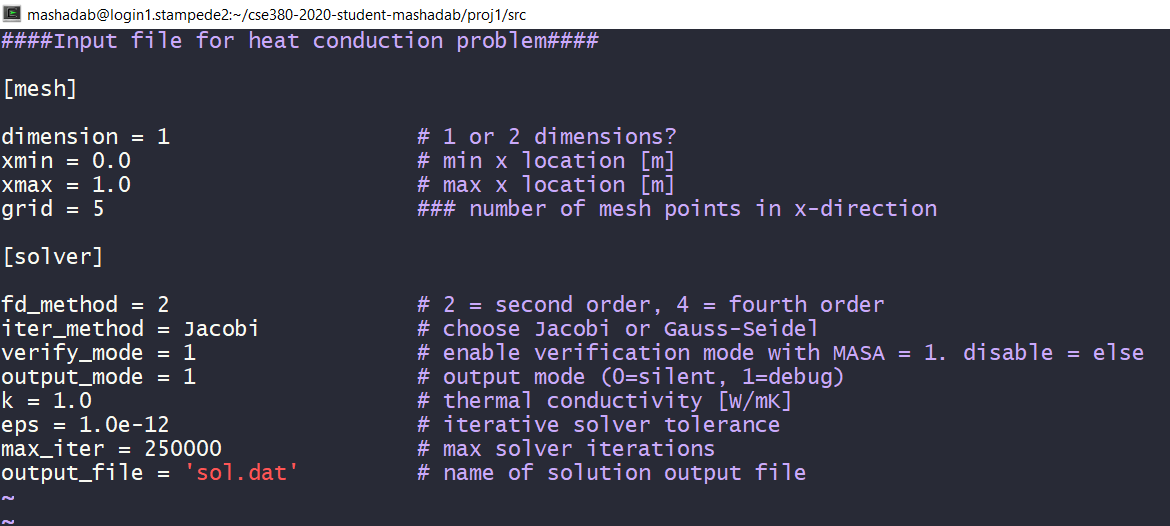
\includegraphics[width=1.3\linewidth]{Project1photos/inputfile.png}
    \caption{Example of inputfile with debug and verification modes on for Jacobi method, order 2, dimension 1 with $N=5$}
    \label{fig:3}
\end{figure}

\subsubsection{Verification mode}:
The verification mode is switched on in the input file {\tt{input\_file.dat}} by {\tt{verify\_mode=1}}. It is off for every other input. The verification mode provides the $L_2$ norm of the error in temperatures $T$ with respect to the exact temperatures provided by {\tt{MASA}} library. An example of the output with debug mode off and verification mode on for Jacobi method, order 2, dimension 1 with $N=5$ is given in Figure \ref{fig:4}.

\begin{figure}[htbp!]
\centering
    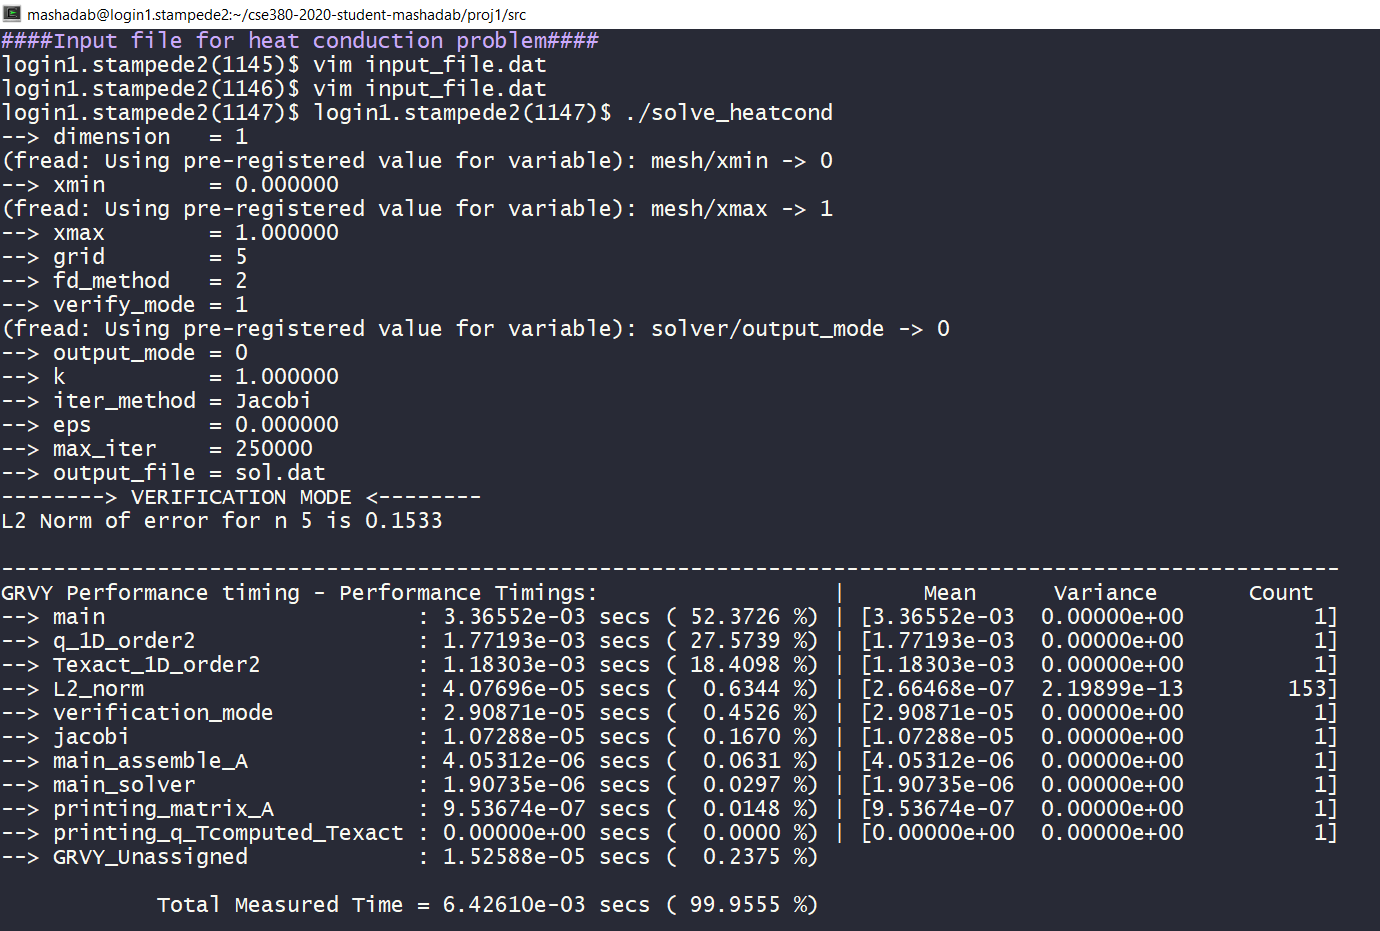
\includegraphics[width=1.3\linewidth]{Project1photos/verification.png}
    \caption{Example of output for verification mode on with Jacobi method, order 2, dimension 1 with $N=5$.}
    \label{fig:4}
\end{figure}

\subsubsection{Debug mode}: 
The debug mode is switched on in the input file {\tt{input\_file.dat}} by {\tt{output\_mode=1}}. It is off for silent mode (=0). The debug output mode provides all the arrays \textbf{A}, \textbf{T}, \textbf{q}, \textbf{T}$_{exact}$ in MATLAB output form for debugging the code. An example of output with debug mode on and verification mode off for Jacobi method, order 2, dimension 1 with $N=5$ is given in Figure \ref{fig:5}.

\begin{figure}[htbp!]
\centering
    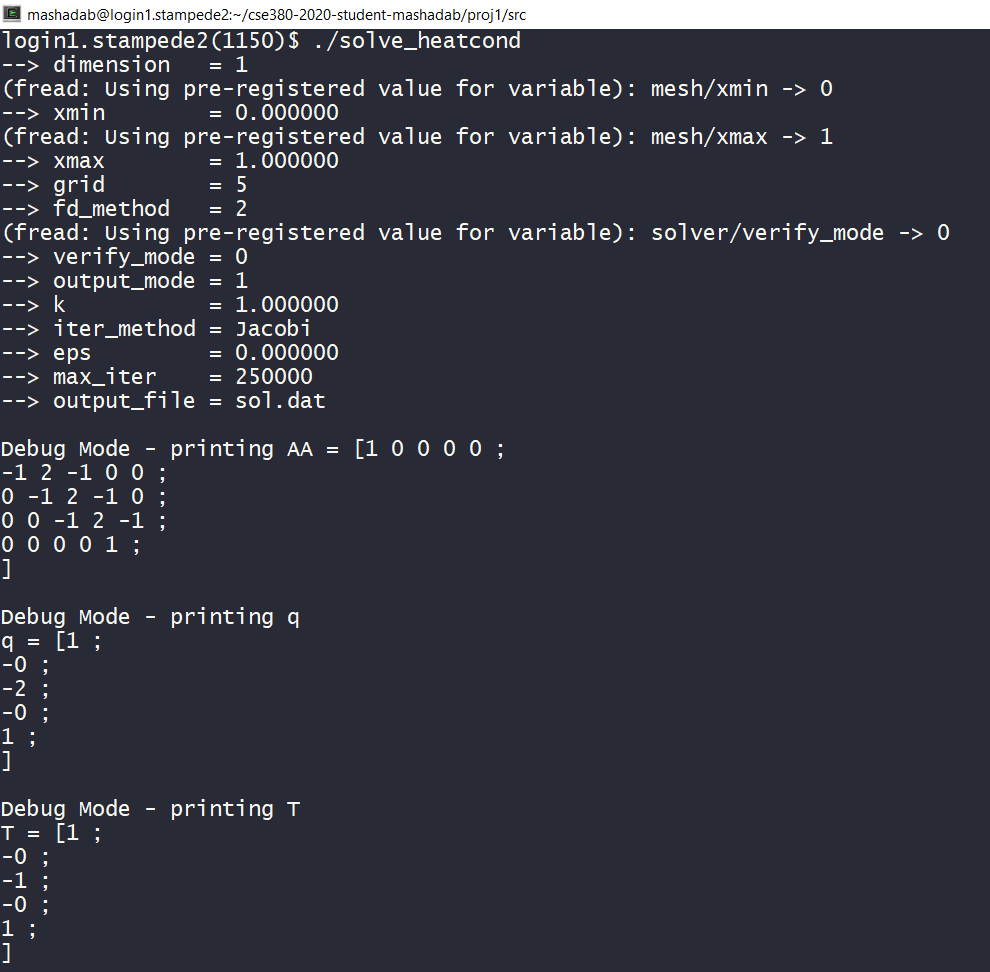
\includegraphics[width=1.1\linewidth]{Project1photos/debug1.png}
    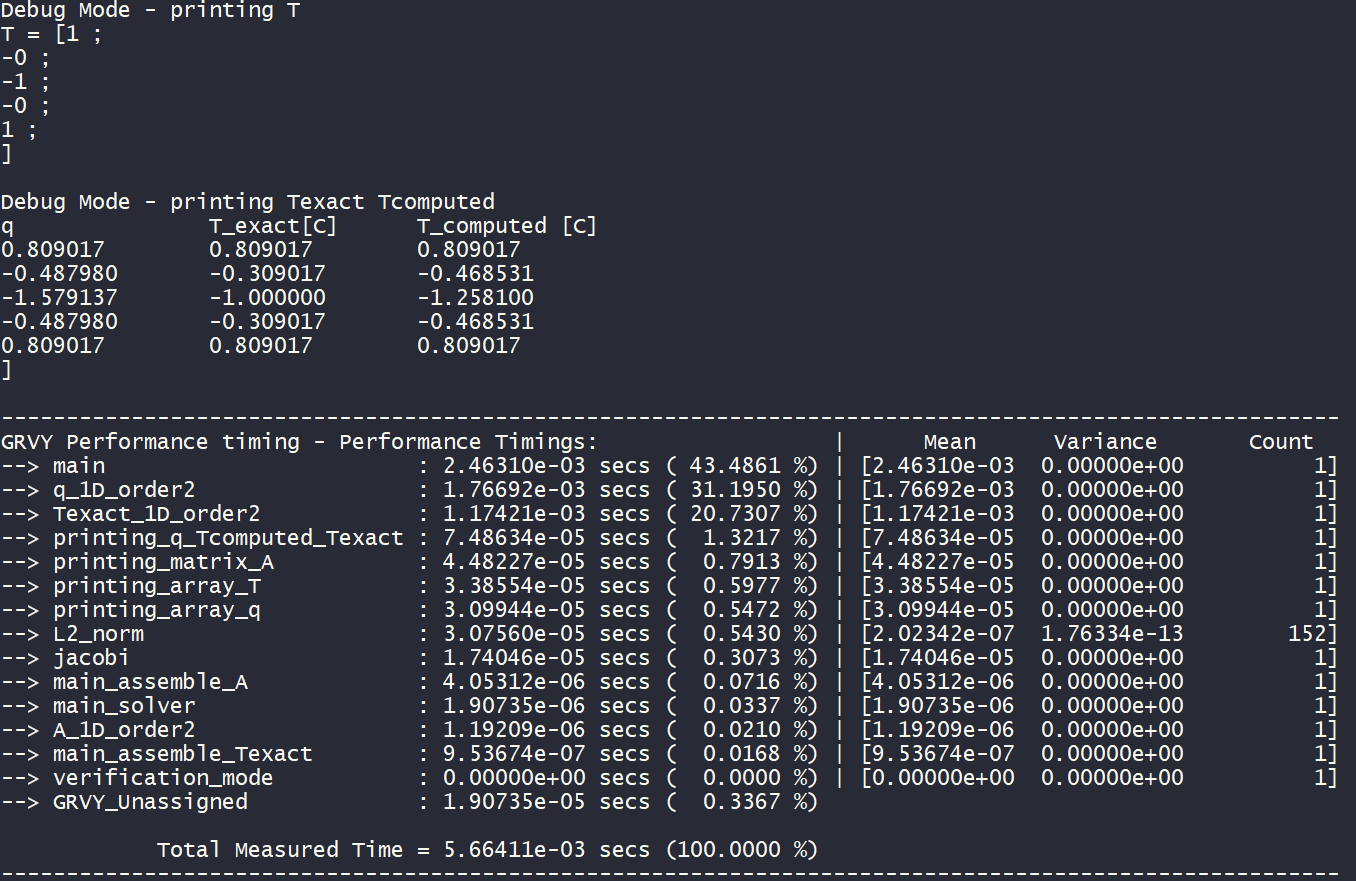
\includegraphics[width=1.1\linewidth, trim= 0 0 0 4cm, clip]{Project1photos/debug2.png}
    \caption{Example of output for verification mode on with Jacobi method, order 2, dimension 1 with $N=5$.}
    \label{fig:5}
\end{figure}

\section{Software testing}
\subsection{Verification testing}
The code is working fine where we get the $L_2$ norm of error which reduces with a rise in grid cells $N$ and we achieve the desired order of convergence. An example of the verification test is shown in Figure \ref{fig:6}.

\begin{figure}[htbp!]
\centering
    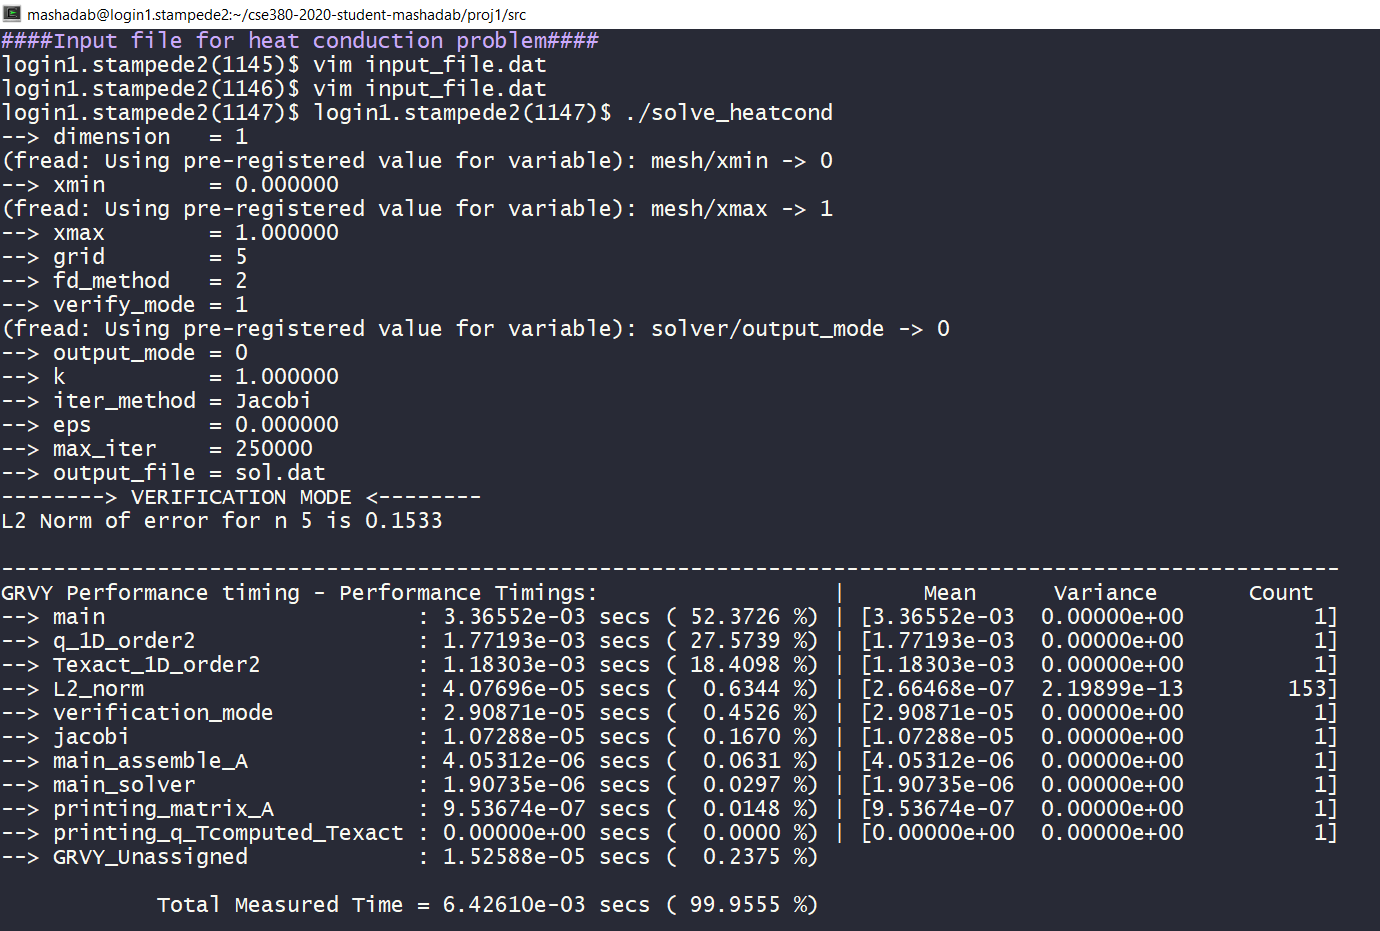
\includegraphics[width=1.3\linewidth]{Project1photos/verification.png}
    \caption{Example of output for verification mode on with Jacobi method, order 2, dimension 1 with $N=5$.}
    \label{fig:6}
\end{figure}

\textbf{Order of convergence analysis}:
\begin{enumerate}
    \item Jacobi: The solver did not converge for fourth order central differencing, so we will only show the results for second order finite differencing in both 1D and 2D. We achieved desired order of convergence as shown in Figure \ref{fig:convjacobi}.
    
\begin{figure}[htbp!] 
\begin{minipage}[]{\linewidth}
%\vspace{-15mm}
  \centering
    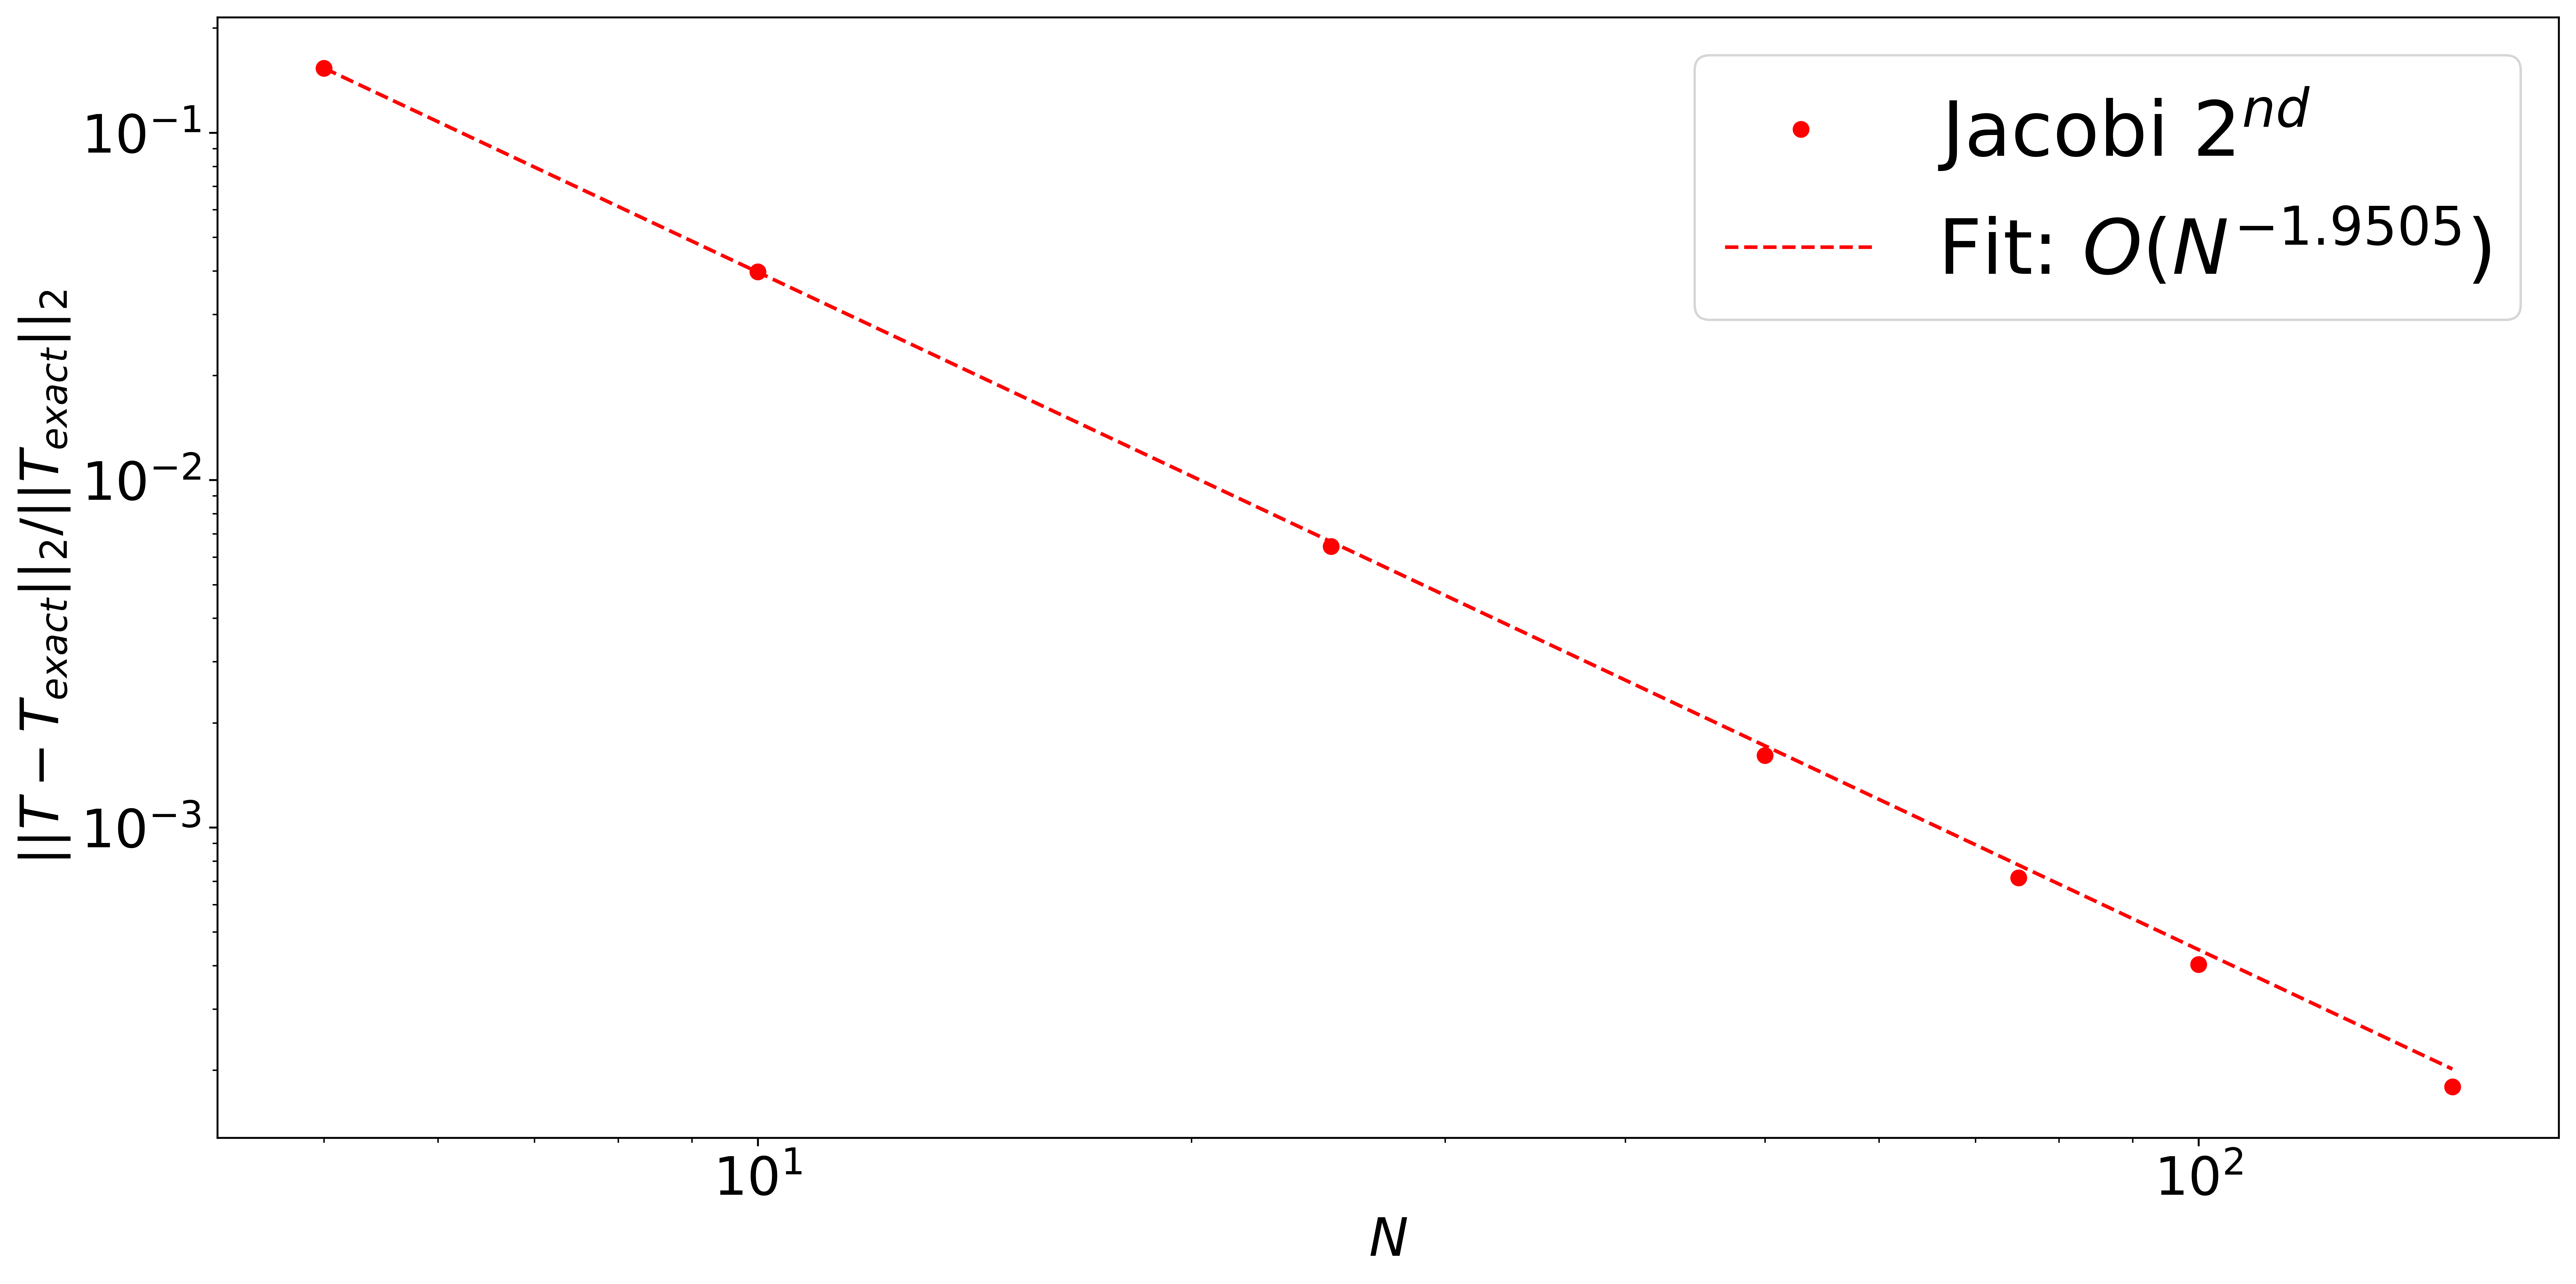
\includegraphics[width=\linewidth,keepaspectratio]{Project1photos/convergence_study_Jacobi_1D.png}
\end{minipage}
\begin{minipage}[htbp!]{\linewidth}
%\vspace{-15mm}
  \centering
    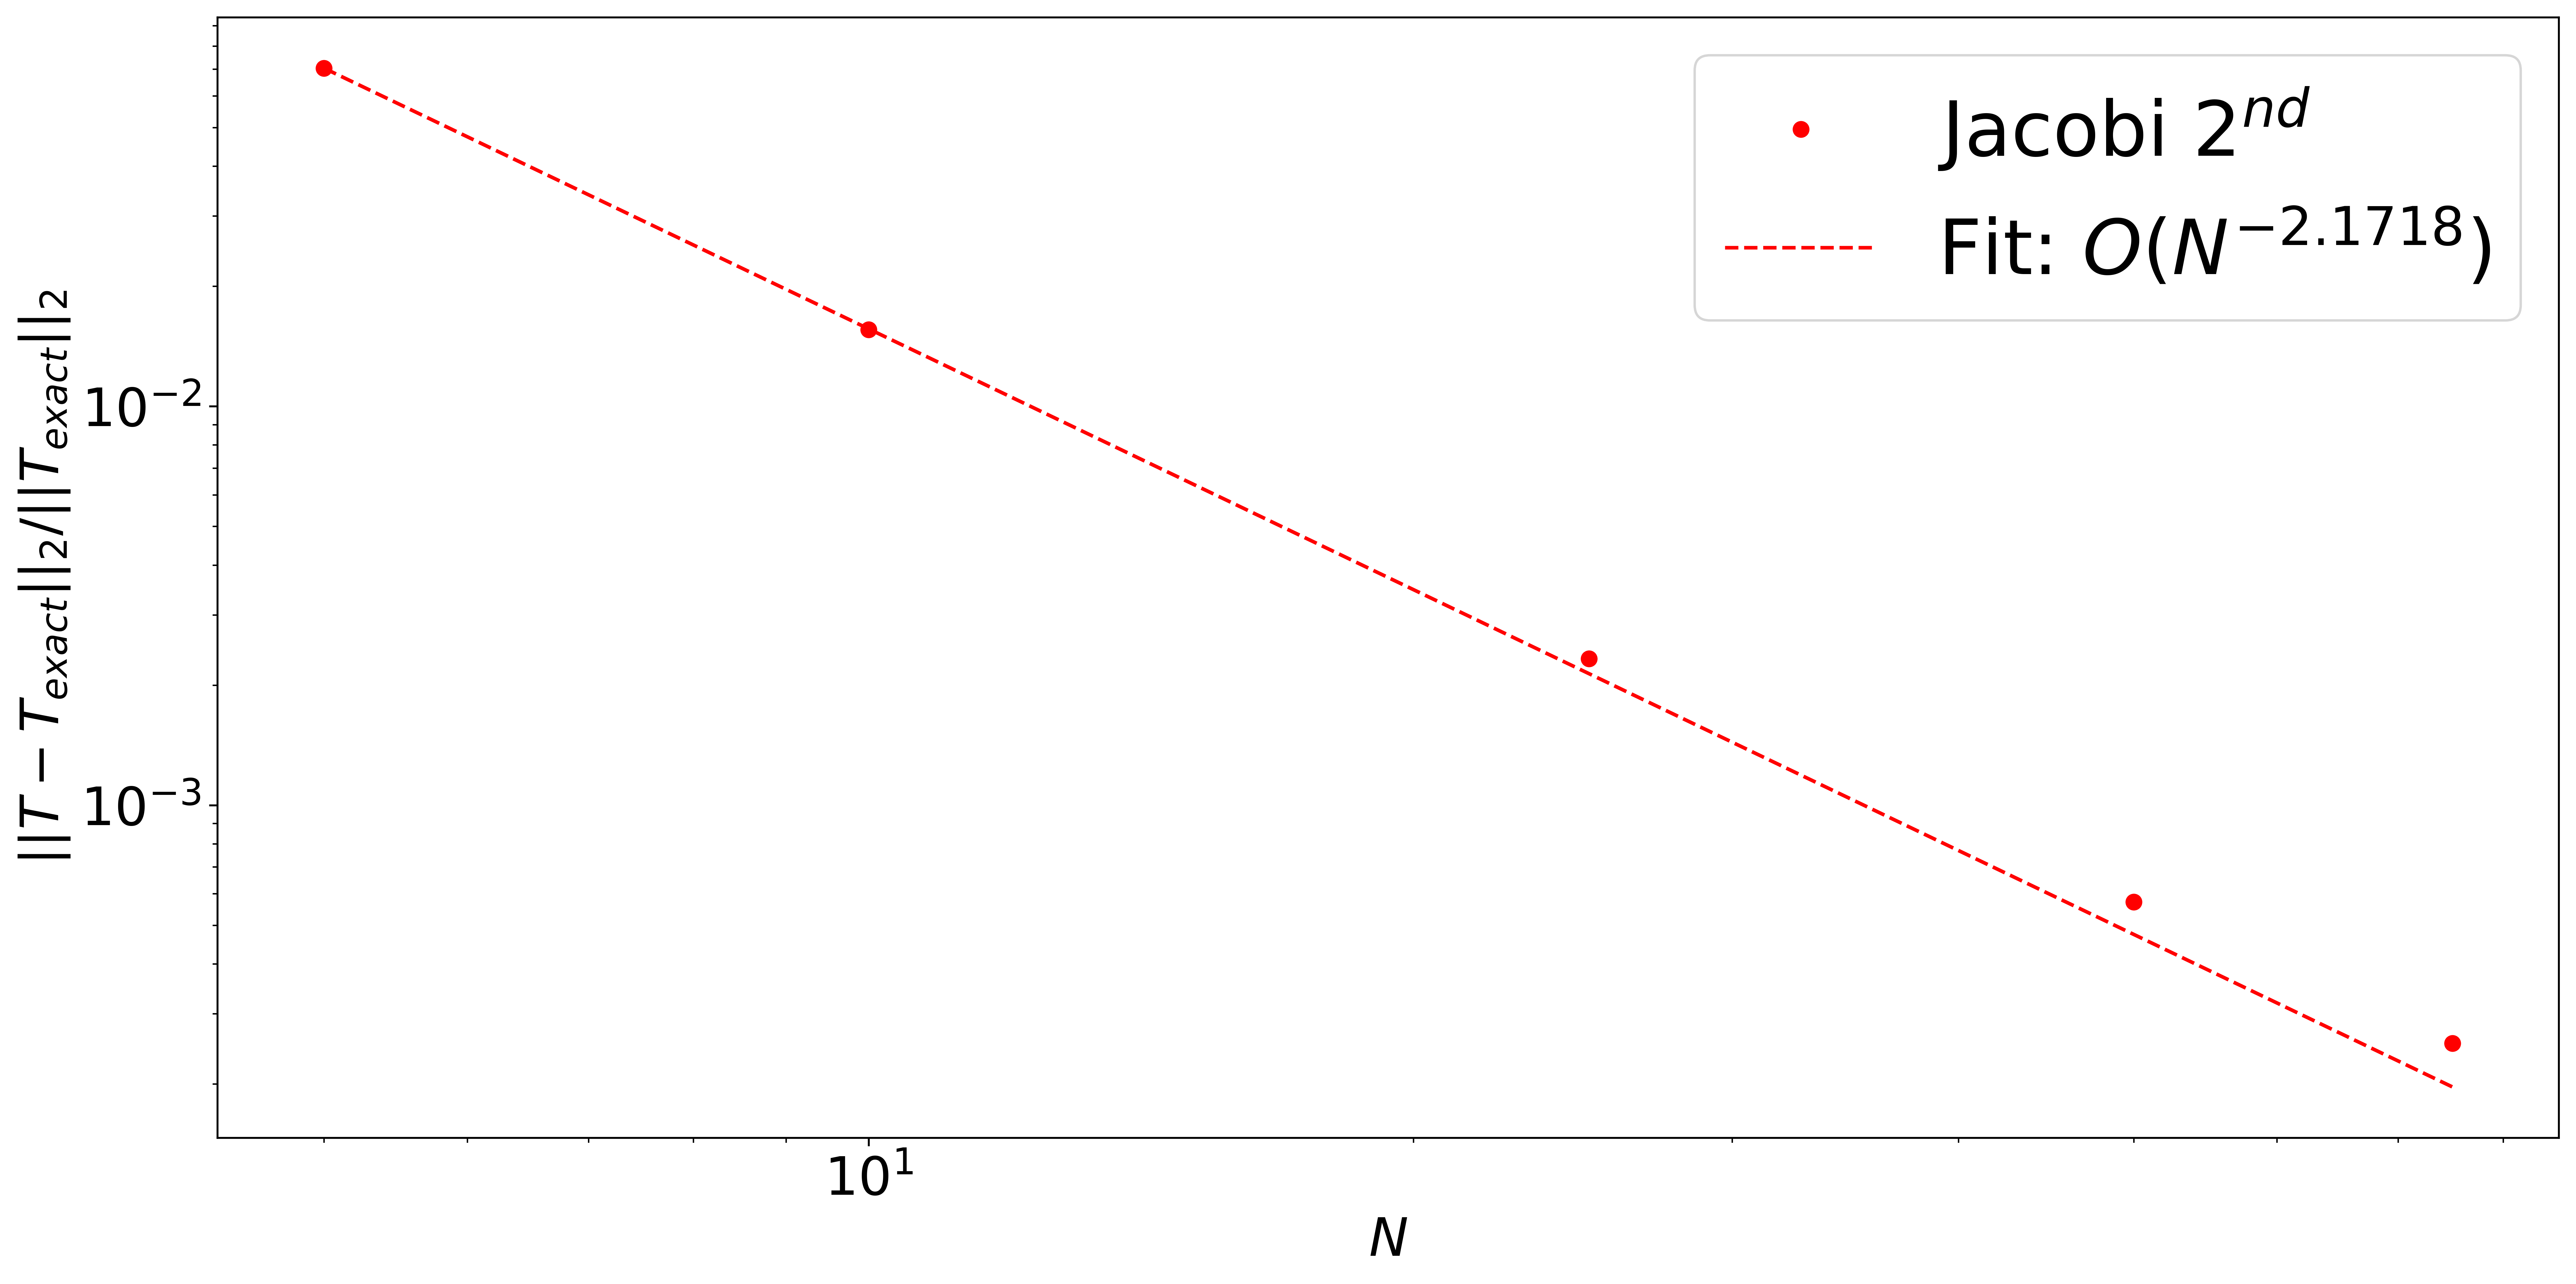
\includegraphics[width=\linewidth,keepaspectratio, trim = 0cm 0cm 0cm 0cm,clip]{Project1photos/convergence_study_Jacobi_2D.png}
\end{minipage}
\caption{Convergence study for 1D (top) and 2D (bottom) cases for second order central differencing using Jacobi iterative solver.} \label{fig:convjacobi}
\end{figure}
    \item Gauss-Seidel: Since Gauss-Seidel took long time to converge, we have gone to $N \times N =75 \times 75$ in 2D but $N = 150$ in 1D. We have achieved desired order of convergence with Gauss-Seidel solver for both second and fourth order finite differencing, as shown in Figure \ref{fig:convGS}.
    
    \begin{figure}[htbp!]
\begin{minipage}[htbp!]{\linewidth}
%\vspace{-15mm}
  \centering
    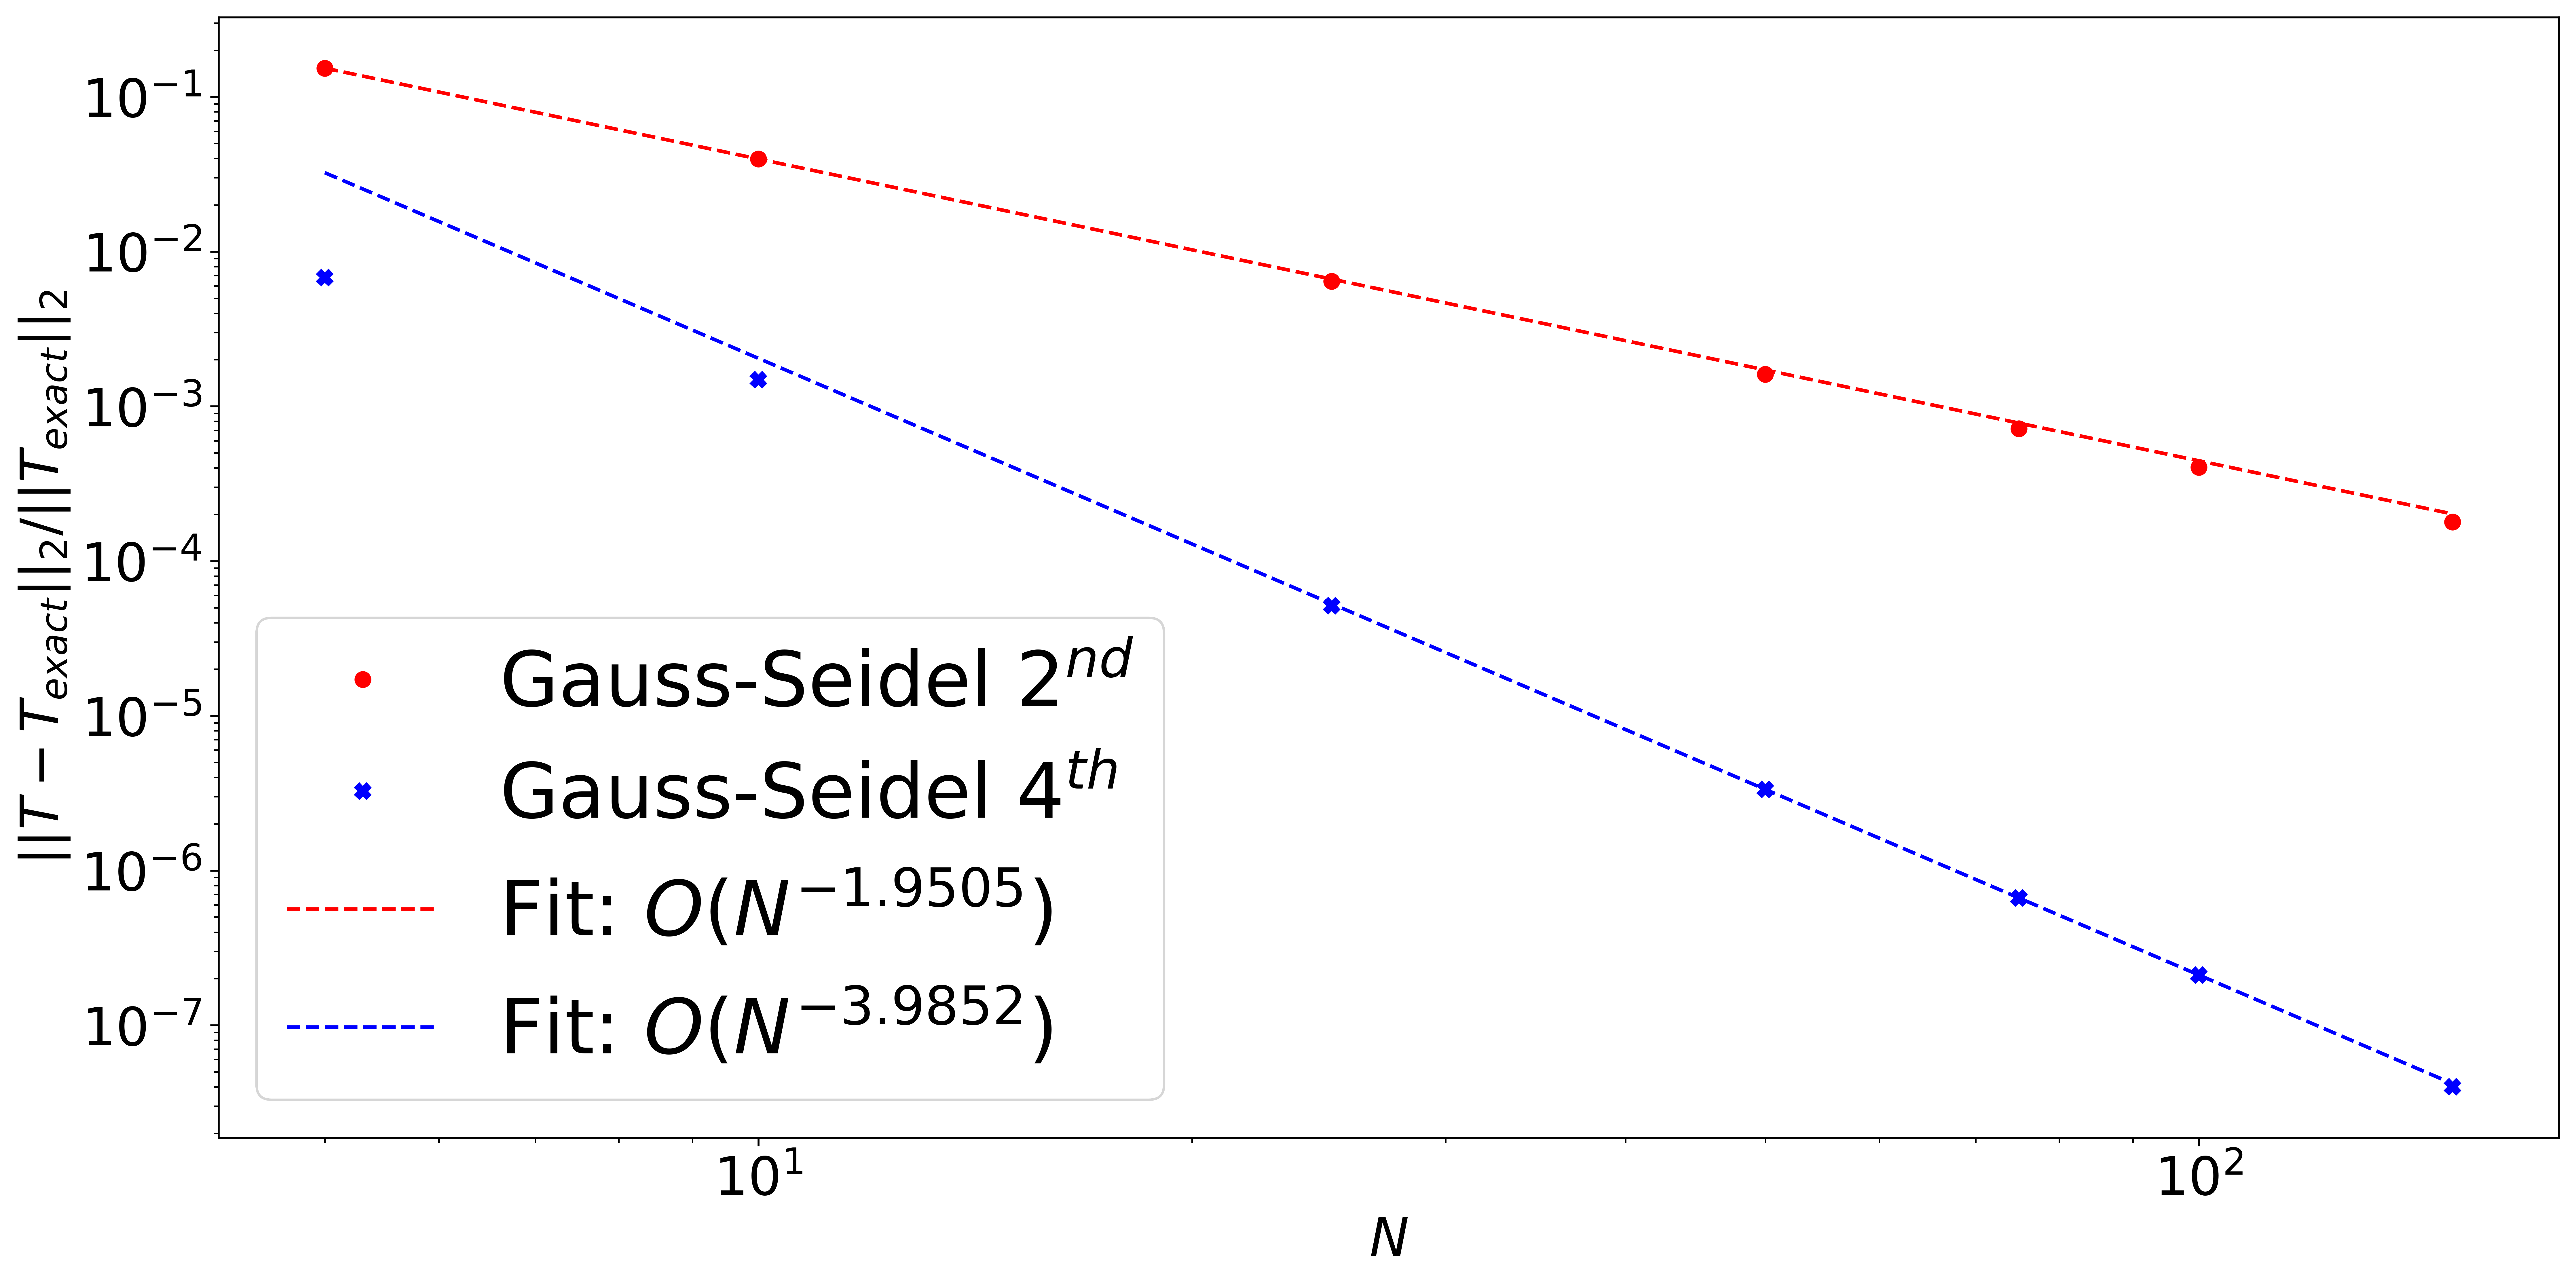
\includegraphics[width=\linewidth,keepaspectratio]{Project1photos/convergence_study_GS_1D.png}
\end{minipage}
\begin{minipage}[htbp!]{\linewidth}
%\vspace{-15mm}
  \centering
    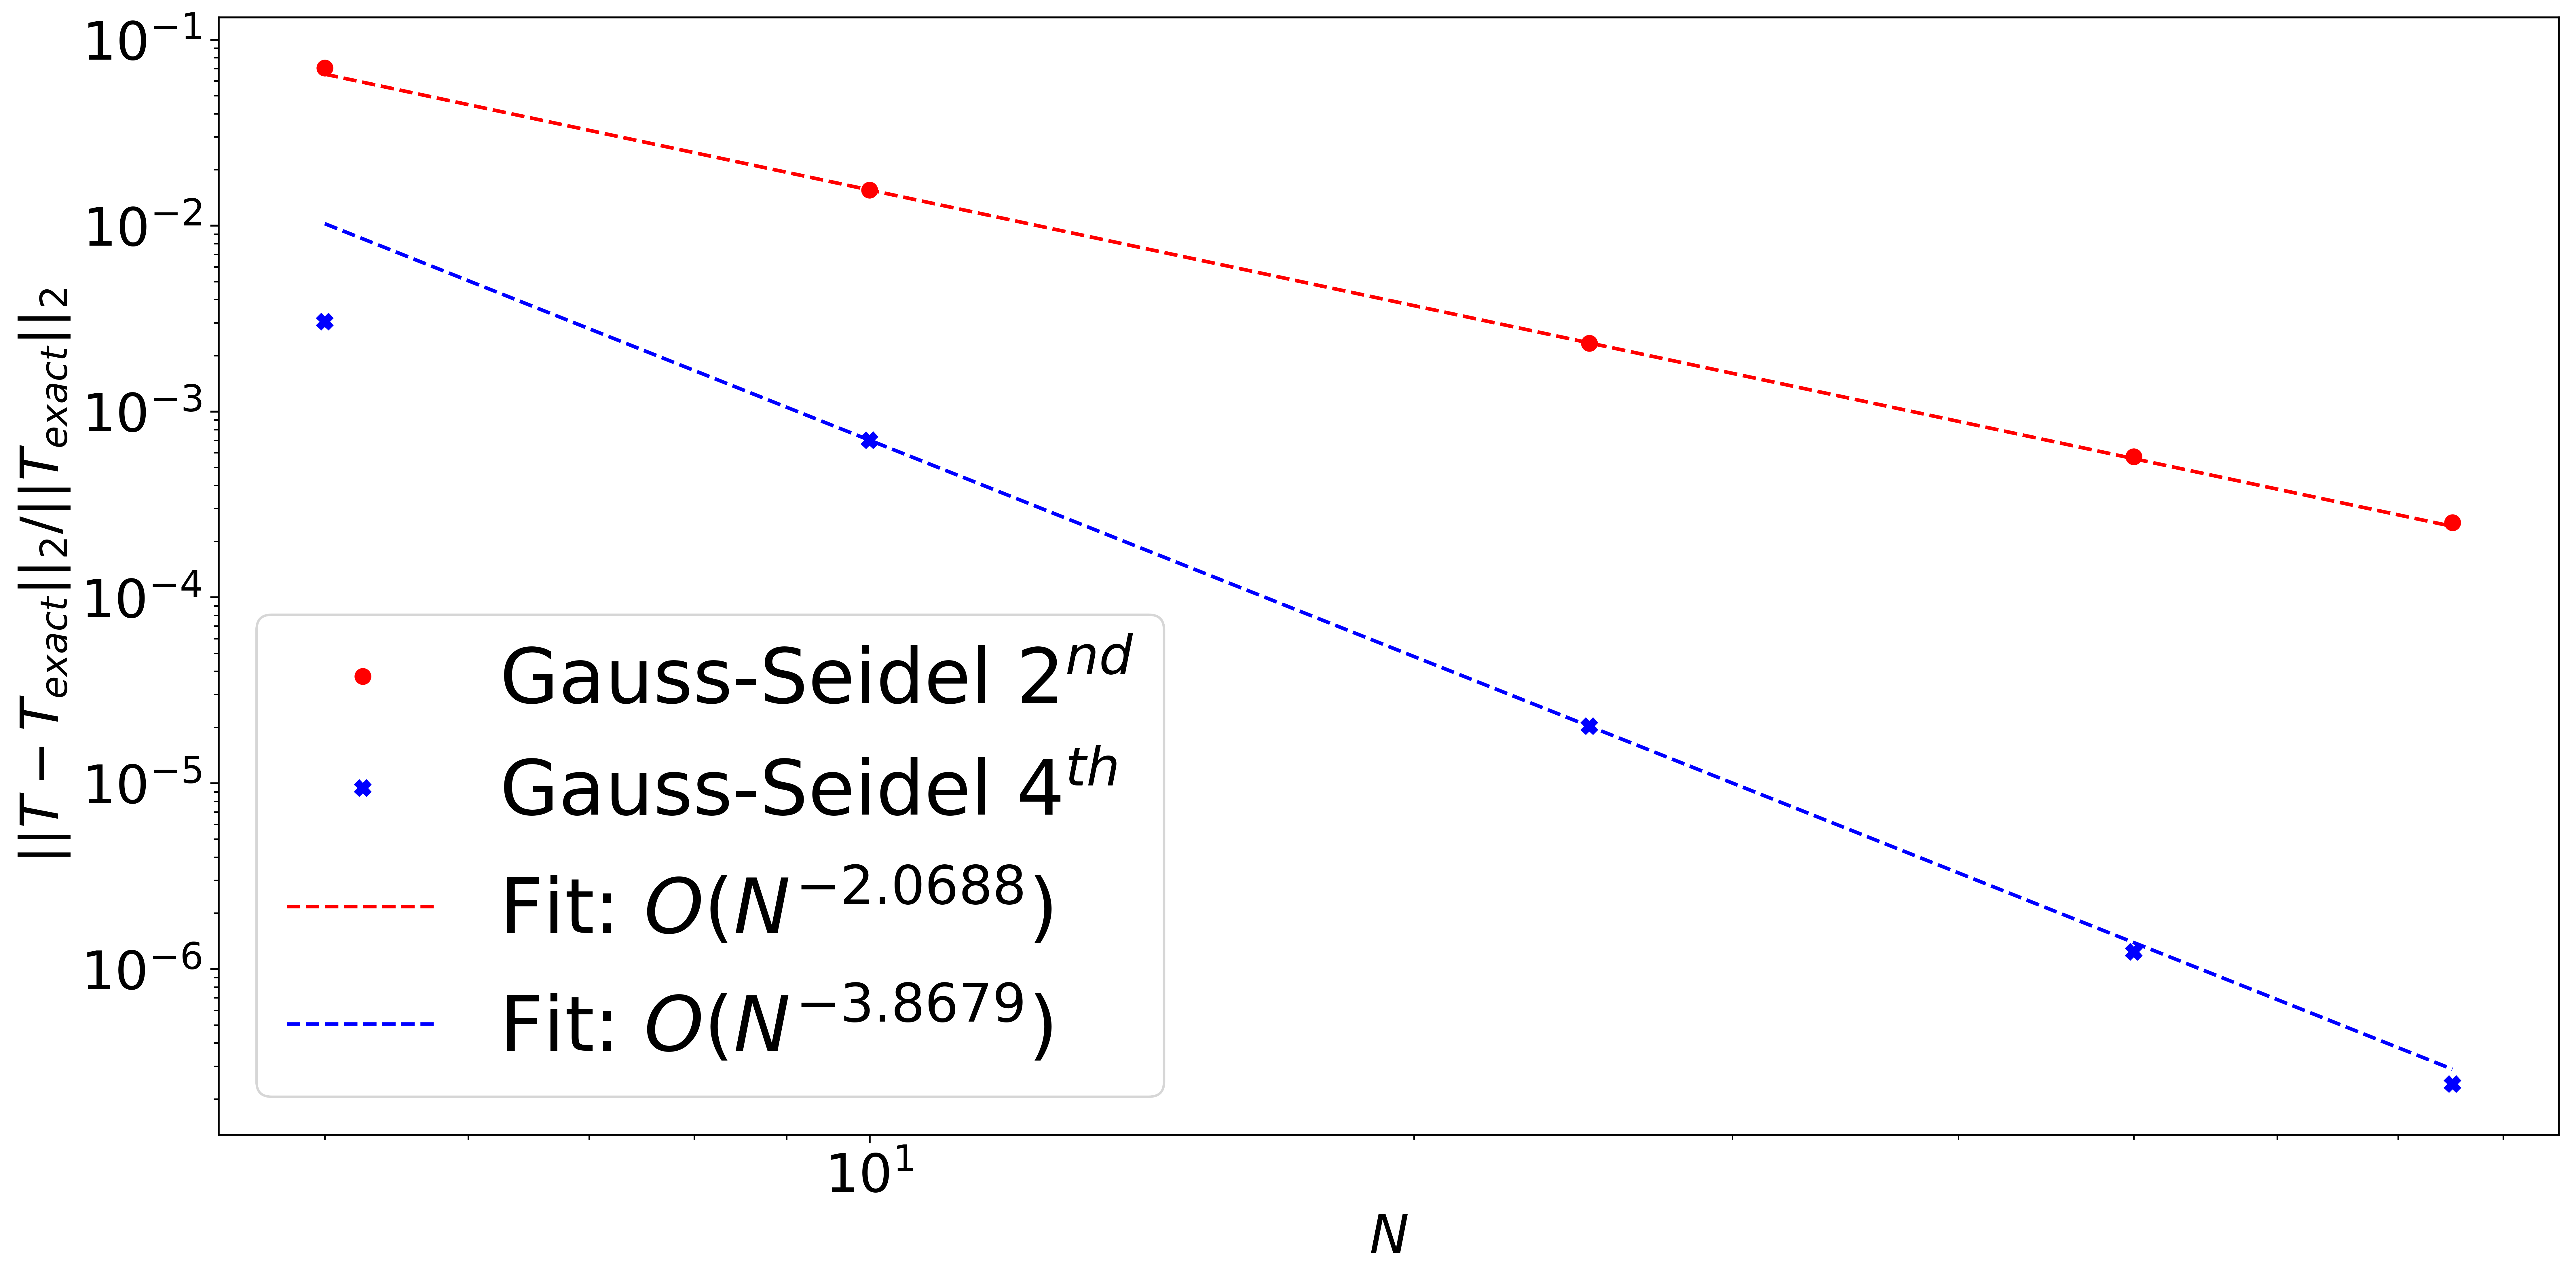
\includegraphics[width=\linewidth,keepaspectratio]{Project1photos/convergence_study_GS_2D.png}
\end{minipage}
\caption{Convergence study for 1D (top) and 2D (bottom) cases for two and fourth order central differencing using Gauss-Seidel iterative solver.} \label{fig:convGS}
\end{figure}
\end{enumerate}

\subsection{Regression testing}
The output of regression testing is given in Figure \ref{fig:7} for the {\tt{make check}} and Figure \ref{fig:8} for the {\tt{./test/rng.sh}}. We successfully passed the 5 tests that we designed, which are: 
\begin{itemize}
    \item Verifying the successful code compilation
    \item Verifying if verification mode runs properly
    \item Verifying if debug mode runs properly
    \item Verifying that the Gauss-Seidel solver matches with reference outputs
    \item Verifying that the Jacobi solver matches with reference outputs
\end{itemize}

\begin{figure}[htbp!]
\centering
    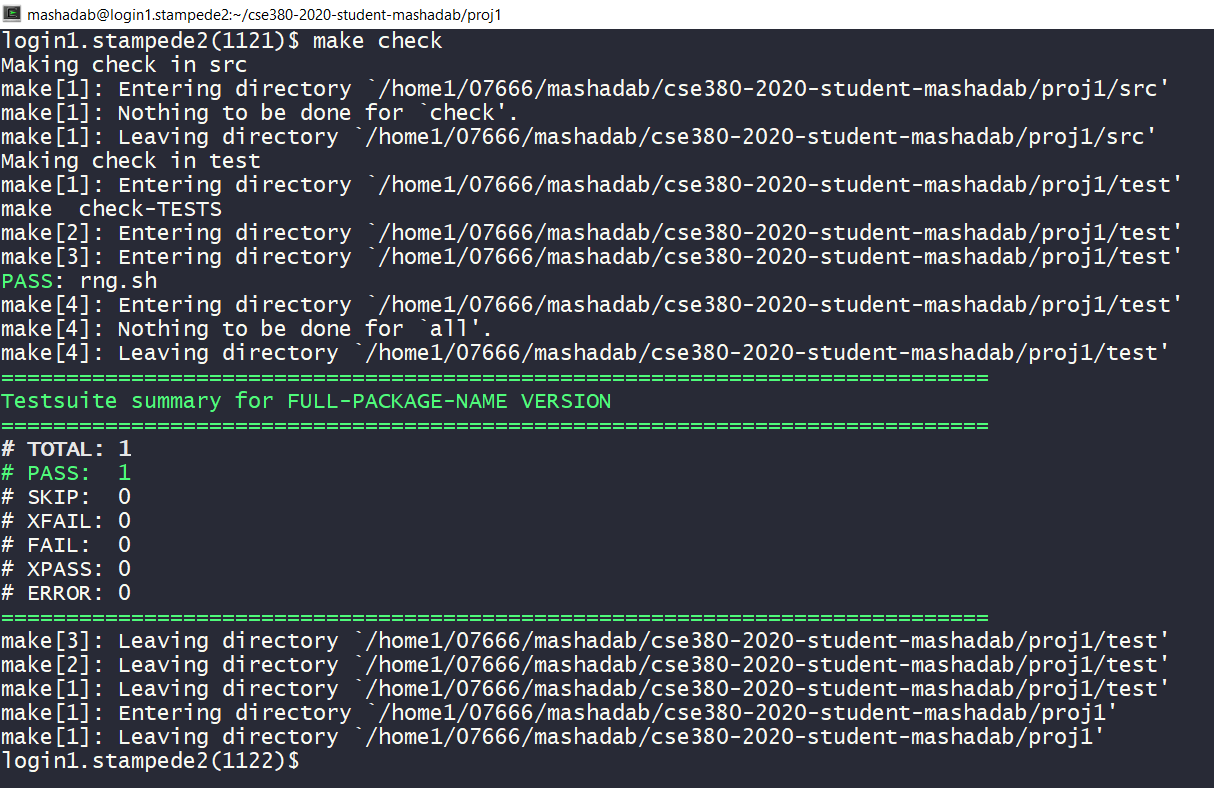
\includegraphics[width=1.3\linewidth]{Project1photos/makecheck.png}
    \caption{Regression testing by running {\tt{make check}} in the main directory. We successfully passed the test {\tt{/test/rng.sh}}, shown in green color.}
    \label{fig:7}
\end{figure}

\begin{figure}[htbp!]
\centering
    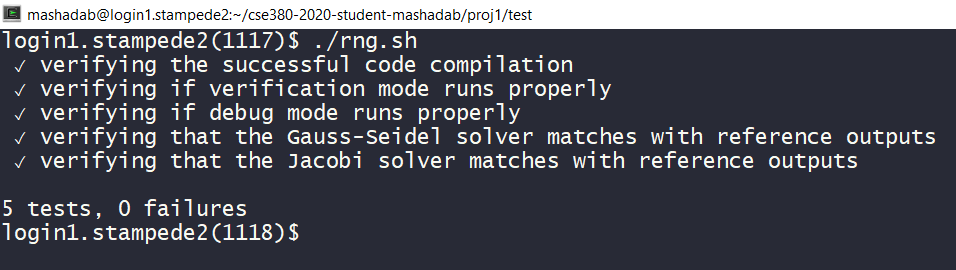
\includegraphics[width=1.3\linewidth]{Project1photos/individualrng.png}
    \caption{Regression testing by running the file {\tt{/test/rng.sh}}.}
    \label{fig:8}
\end{figure}

\subsection{Runtime performance testing}
An example of run time results is given in Figure \ref{fig:9}.
\begin{figure}[htbp!]
\centering
    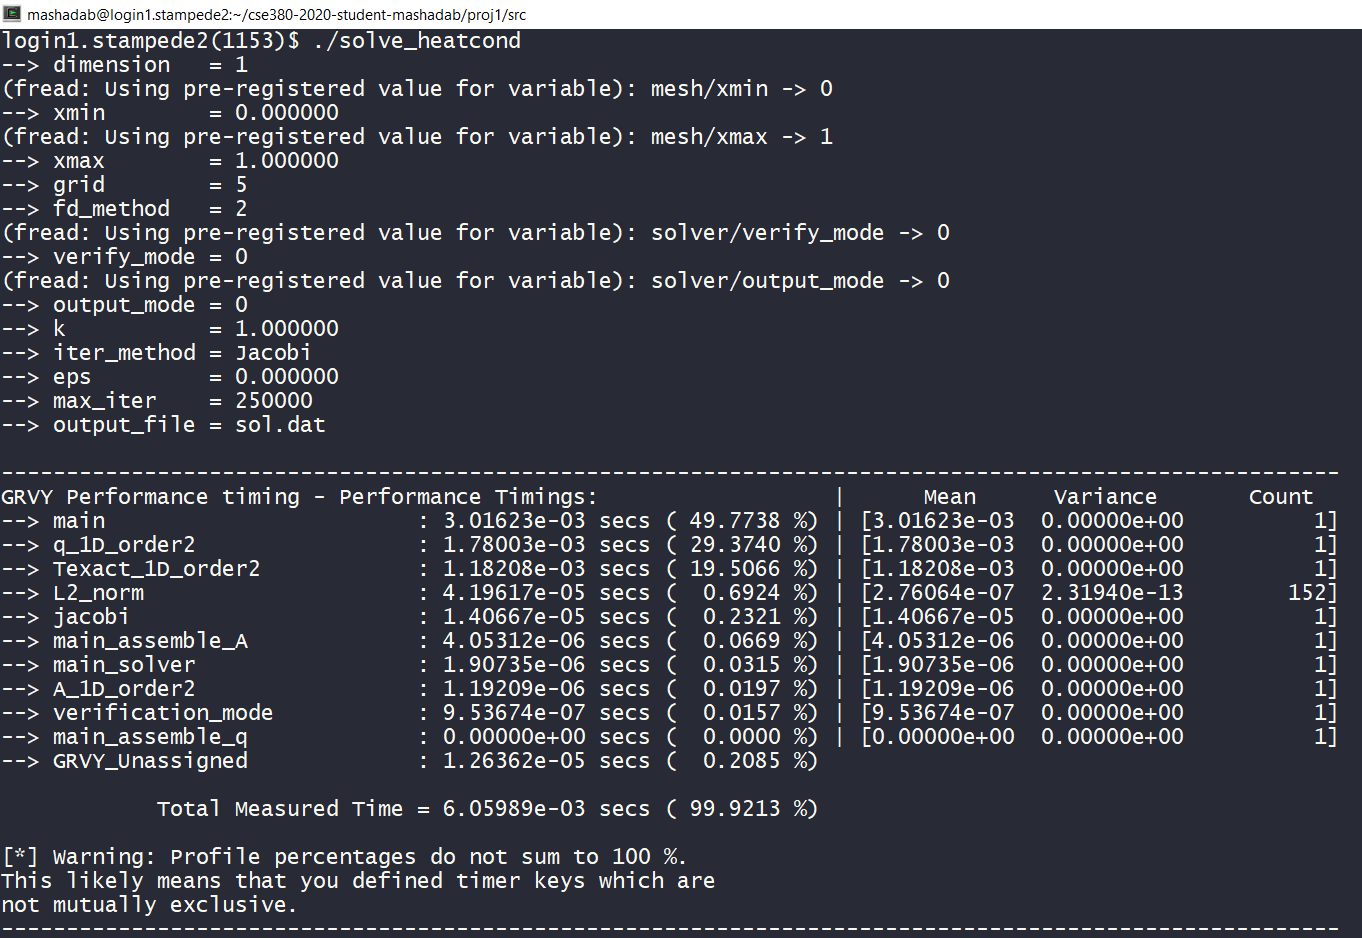
\includegraphics[width=1.3\linewidth]{Project1photos/withoutdebug_verify.png}
    \caption{Example of runtime performance output with Jacobi method, order 2, dimension 1 with $N=5$.}
    \label{fig:9}
\end{figure}

\textbf{Runtime analysis}:
\begin{enumerate}
    \item Jacobi:
The run time increases with $N$, as expected. From Figure \ref{fig:runtimejacobi}, it can be seen that time for 2D case is almost 3 orders of magnitude higher than for 1D case for same $N$ as the number of grids in former is the square of the latter.

\begin{figure}[htbp!] 
\begin{minipage}[]{\linewidth}
%\vspace{-15mm}
  \centering
    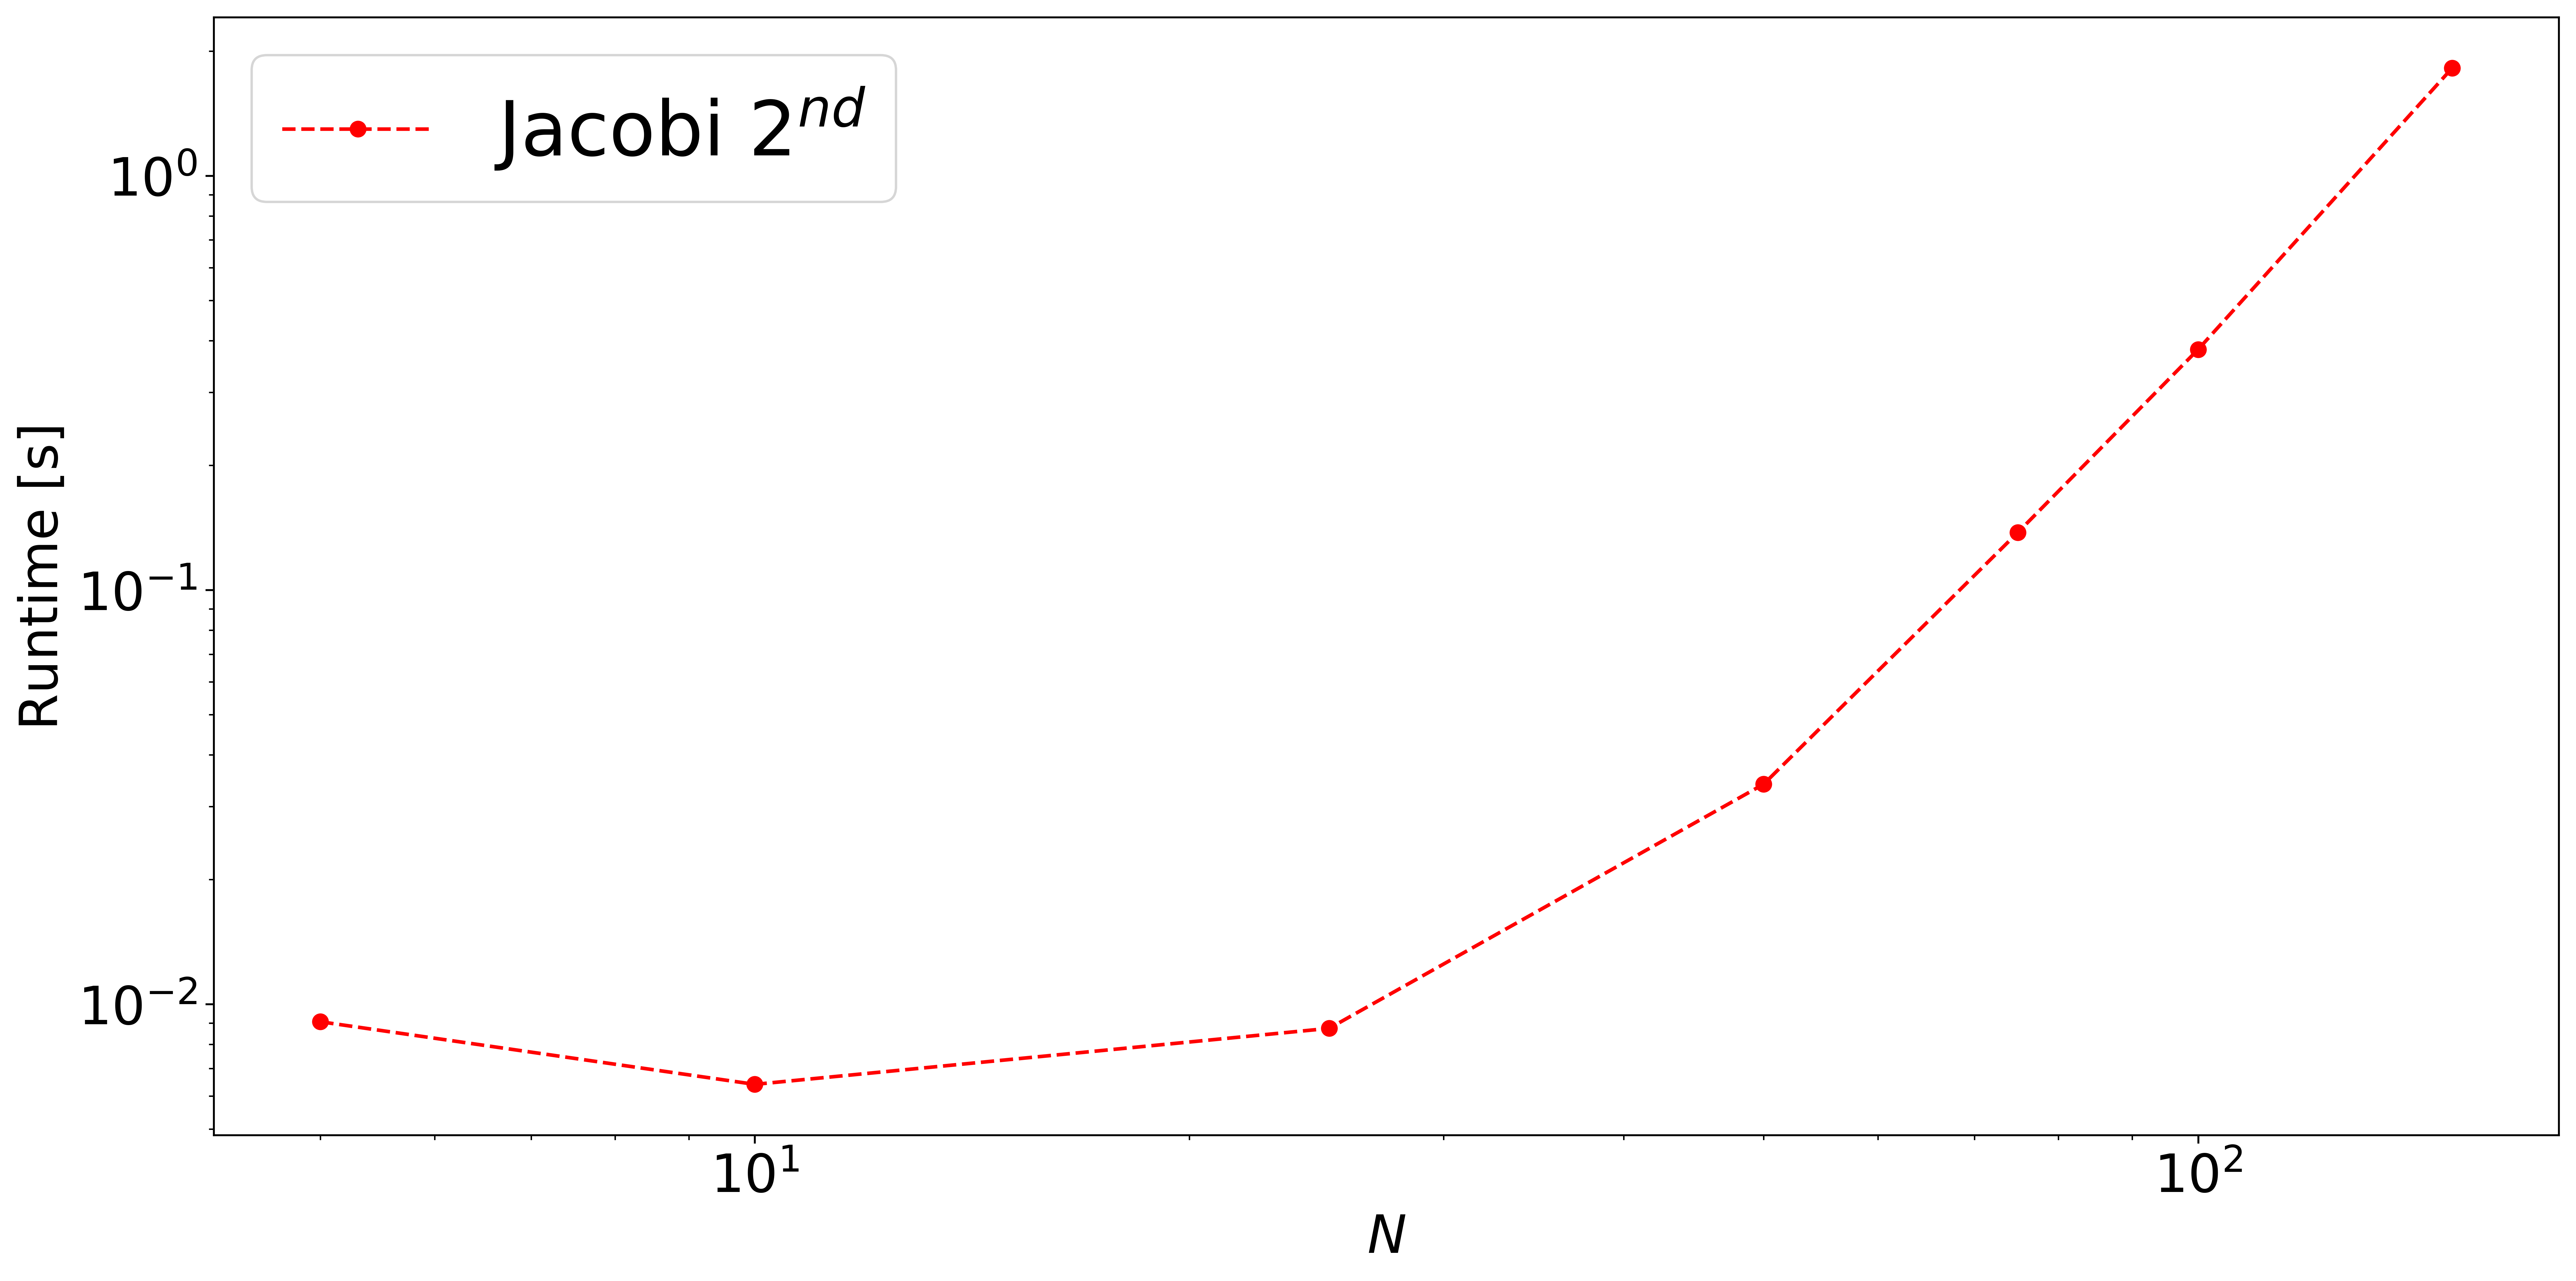
\includegraphics[width=\linewidth,keepaspectratio]{Project1photos/runtime_Jacobi_1D.png}
\end{minipage}
\begin{minipage}[htbp!]{\linewidth}
%\vspace{-15mm}
  \centering
    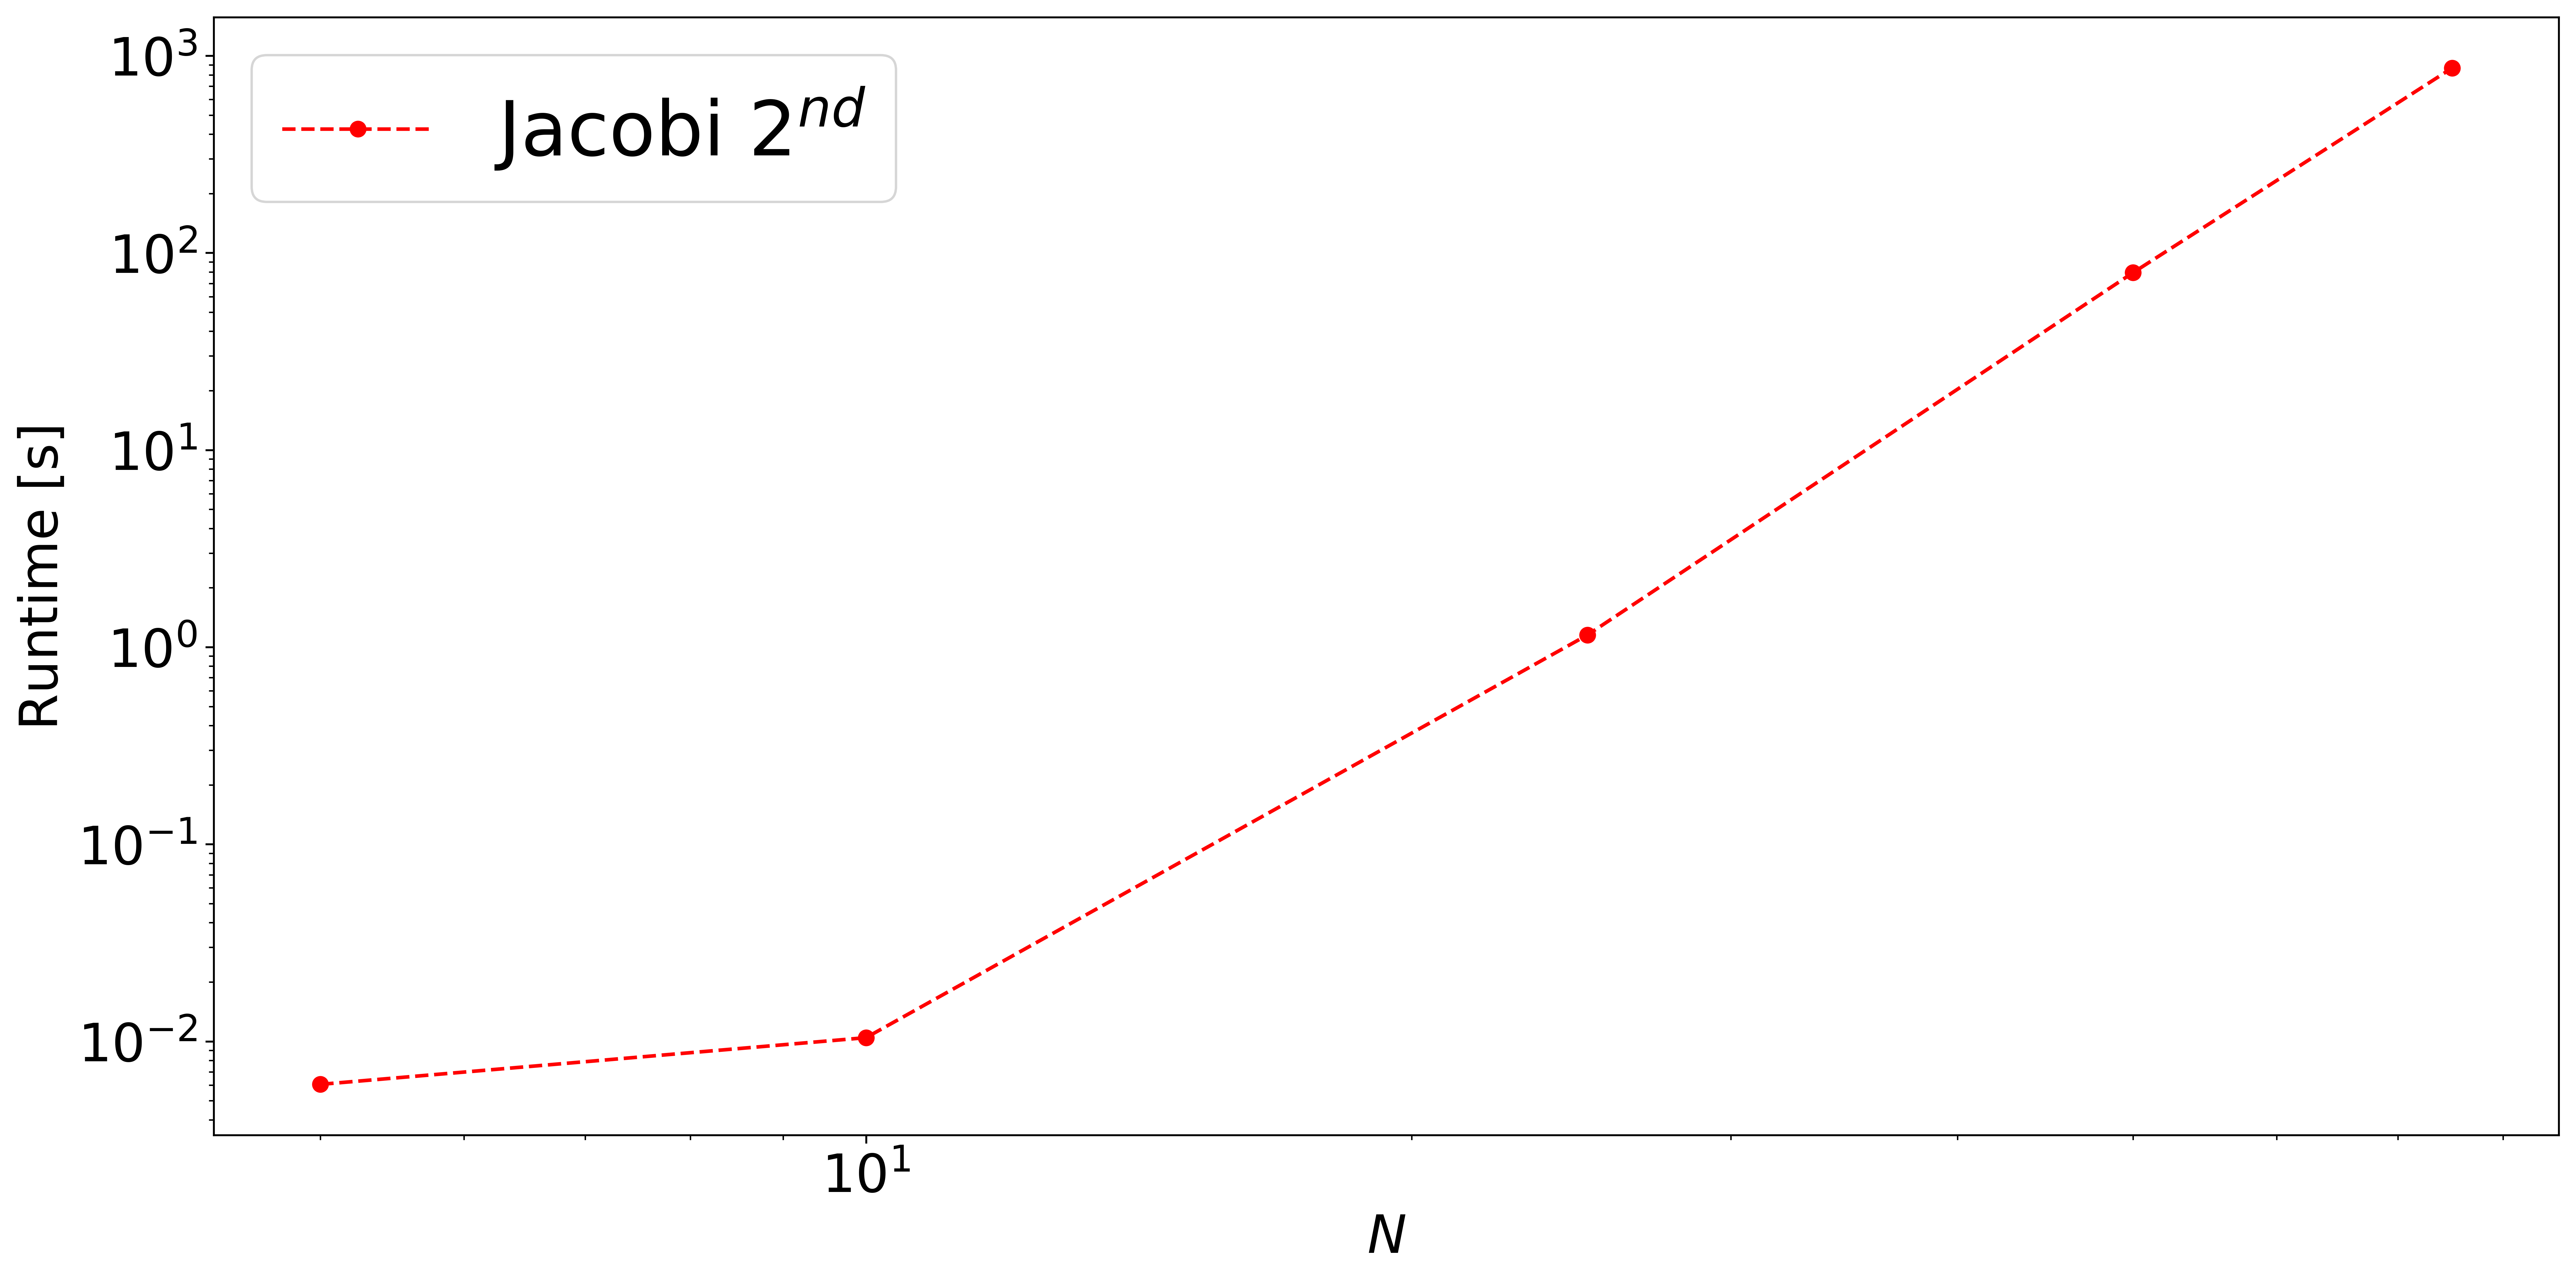
\includegraphics[width=\linewidth,keepaspectratio, trim = 0cm 0cm 0cm 0cm,clip]{Project1photos/runtime_Jacobi_2D.png}
\end{minipage}
\caption{CPU Runtimes for 1D (top) and 2D (bottom) cases for second order central differencing using Jacobi iterative solver using 1 skx node and 48 cores on Stampede 2 supercomputer at TACC.} \label{fig:runtimejacobi}
\end{figure}
    
    \item Gauss-Seidel:
The run time increases with $N$, as expected. From Figure \ref{fig:runtimeGS}, it can be seen that time for 2D case is almost 2 orders of magnitude higher than for 1D case for same $N$ as the number of grids in former is the square of the latter. Also, we can observe that the time for second and fourth order central differencing are the very similar, although the values are little higher for latter. But interestingly, it busts the myth that higher order methods are more expensive. By increasing the order, the errors are reducing by $N^{-4}$ even though the computational cost is very similar, proving the utility of high order methods.

\begin{figure}[htbp!] 
\begin{minipage}[]{\linewidth}
%\vspace{-15mm}
  \centering
    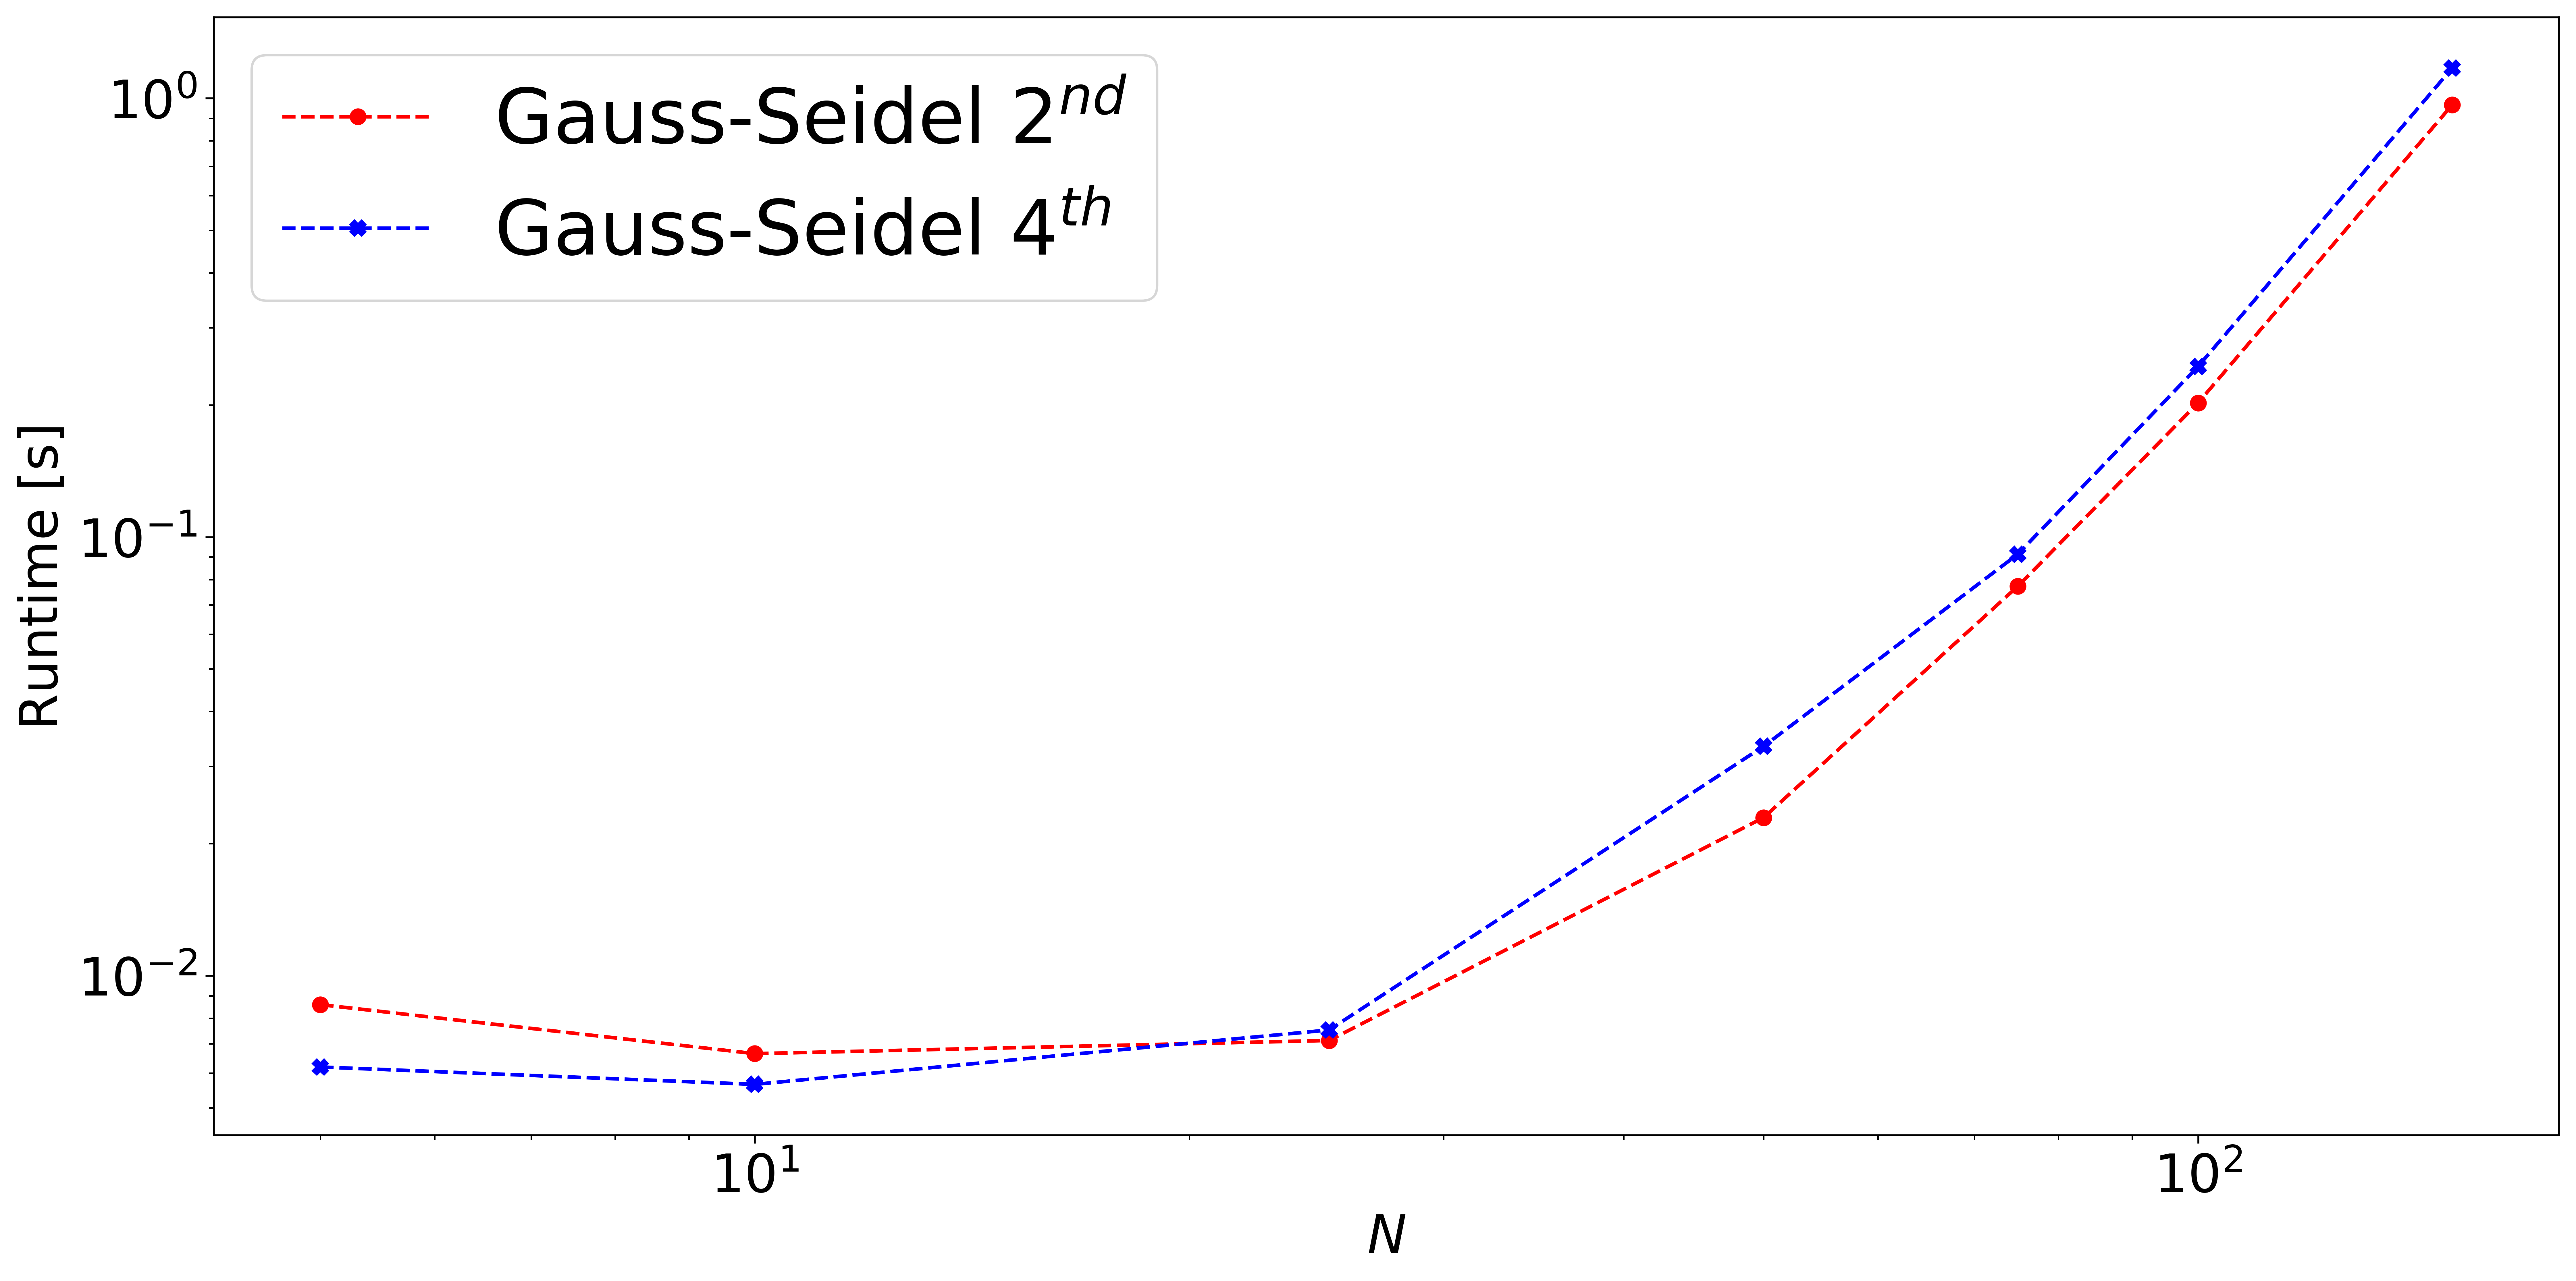
\includegraphics[width=\linewidth,keepaspectratio]{Project1photos/runtime_GS_1D.png}
\end{minipage}
\begin{minipage}[htbp!]{\linewidth}
%\vspace{-15mm}
  \centering
    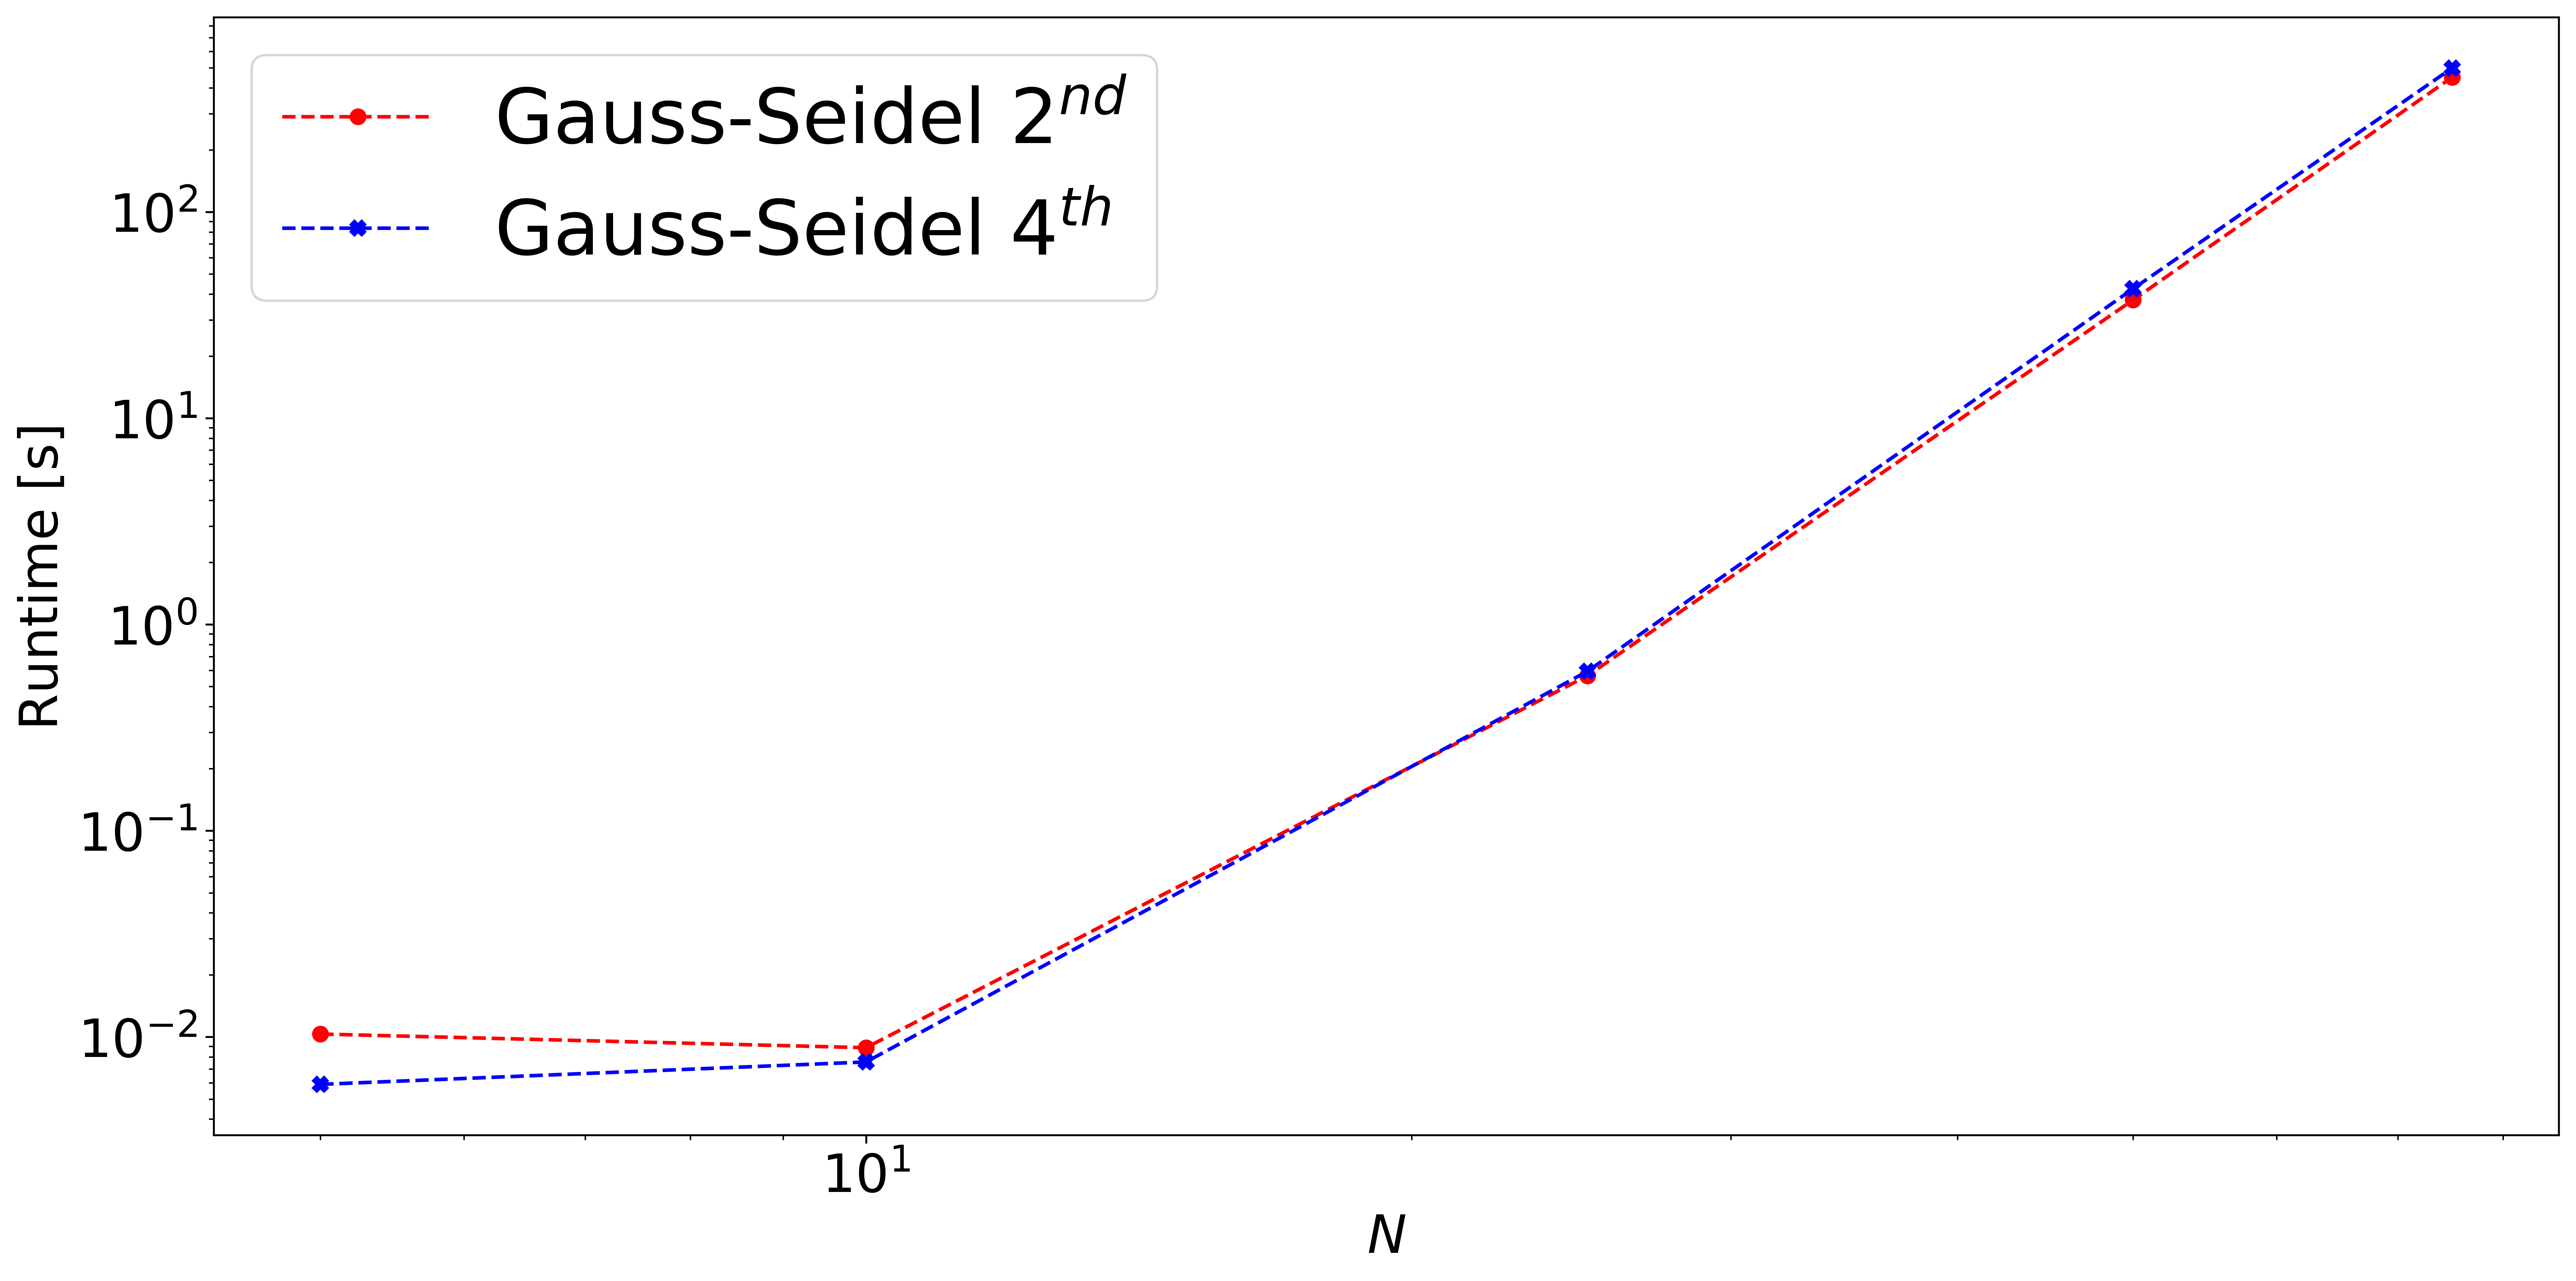
\includegraphics[width=\linewidth,keepaspectratio, trim = 0cm 0cm 0cm 0cm,clip]{Project1photos/runtime_GS_2D.png}
\end{minipage}
\caption{CPU Runtimes for 1D (top) and 2D (bottom) cases for second and fourth order central differencing using Gauss-Seidel iterative solver using 1 node and 48 cores using 1 skx node and 48 cores on Stampede 2 supercomputer at TACC.} \label{fig:runtimeGS}
\end{figure}
\end{enumerate}

\section{Results}
The results for one dimensional tests are given in Figure \ref{fig:plot1D} and for two-dimensional tests are given in Figure \ref{fig:plot2D}.

\begin{figure}[htbp!] 
\begin{minipage}[htbp!]{\linewidth}
%\vspace{-15mm}
  \centering
    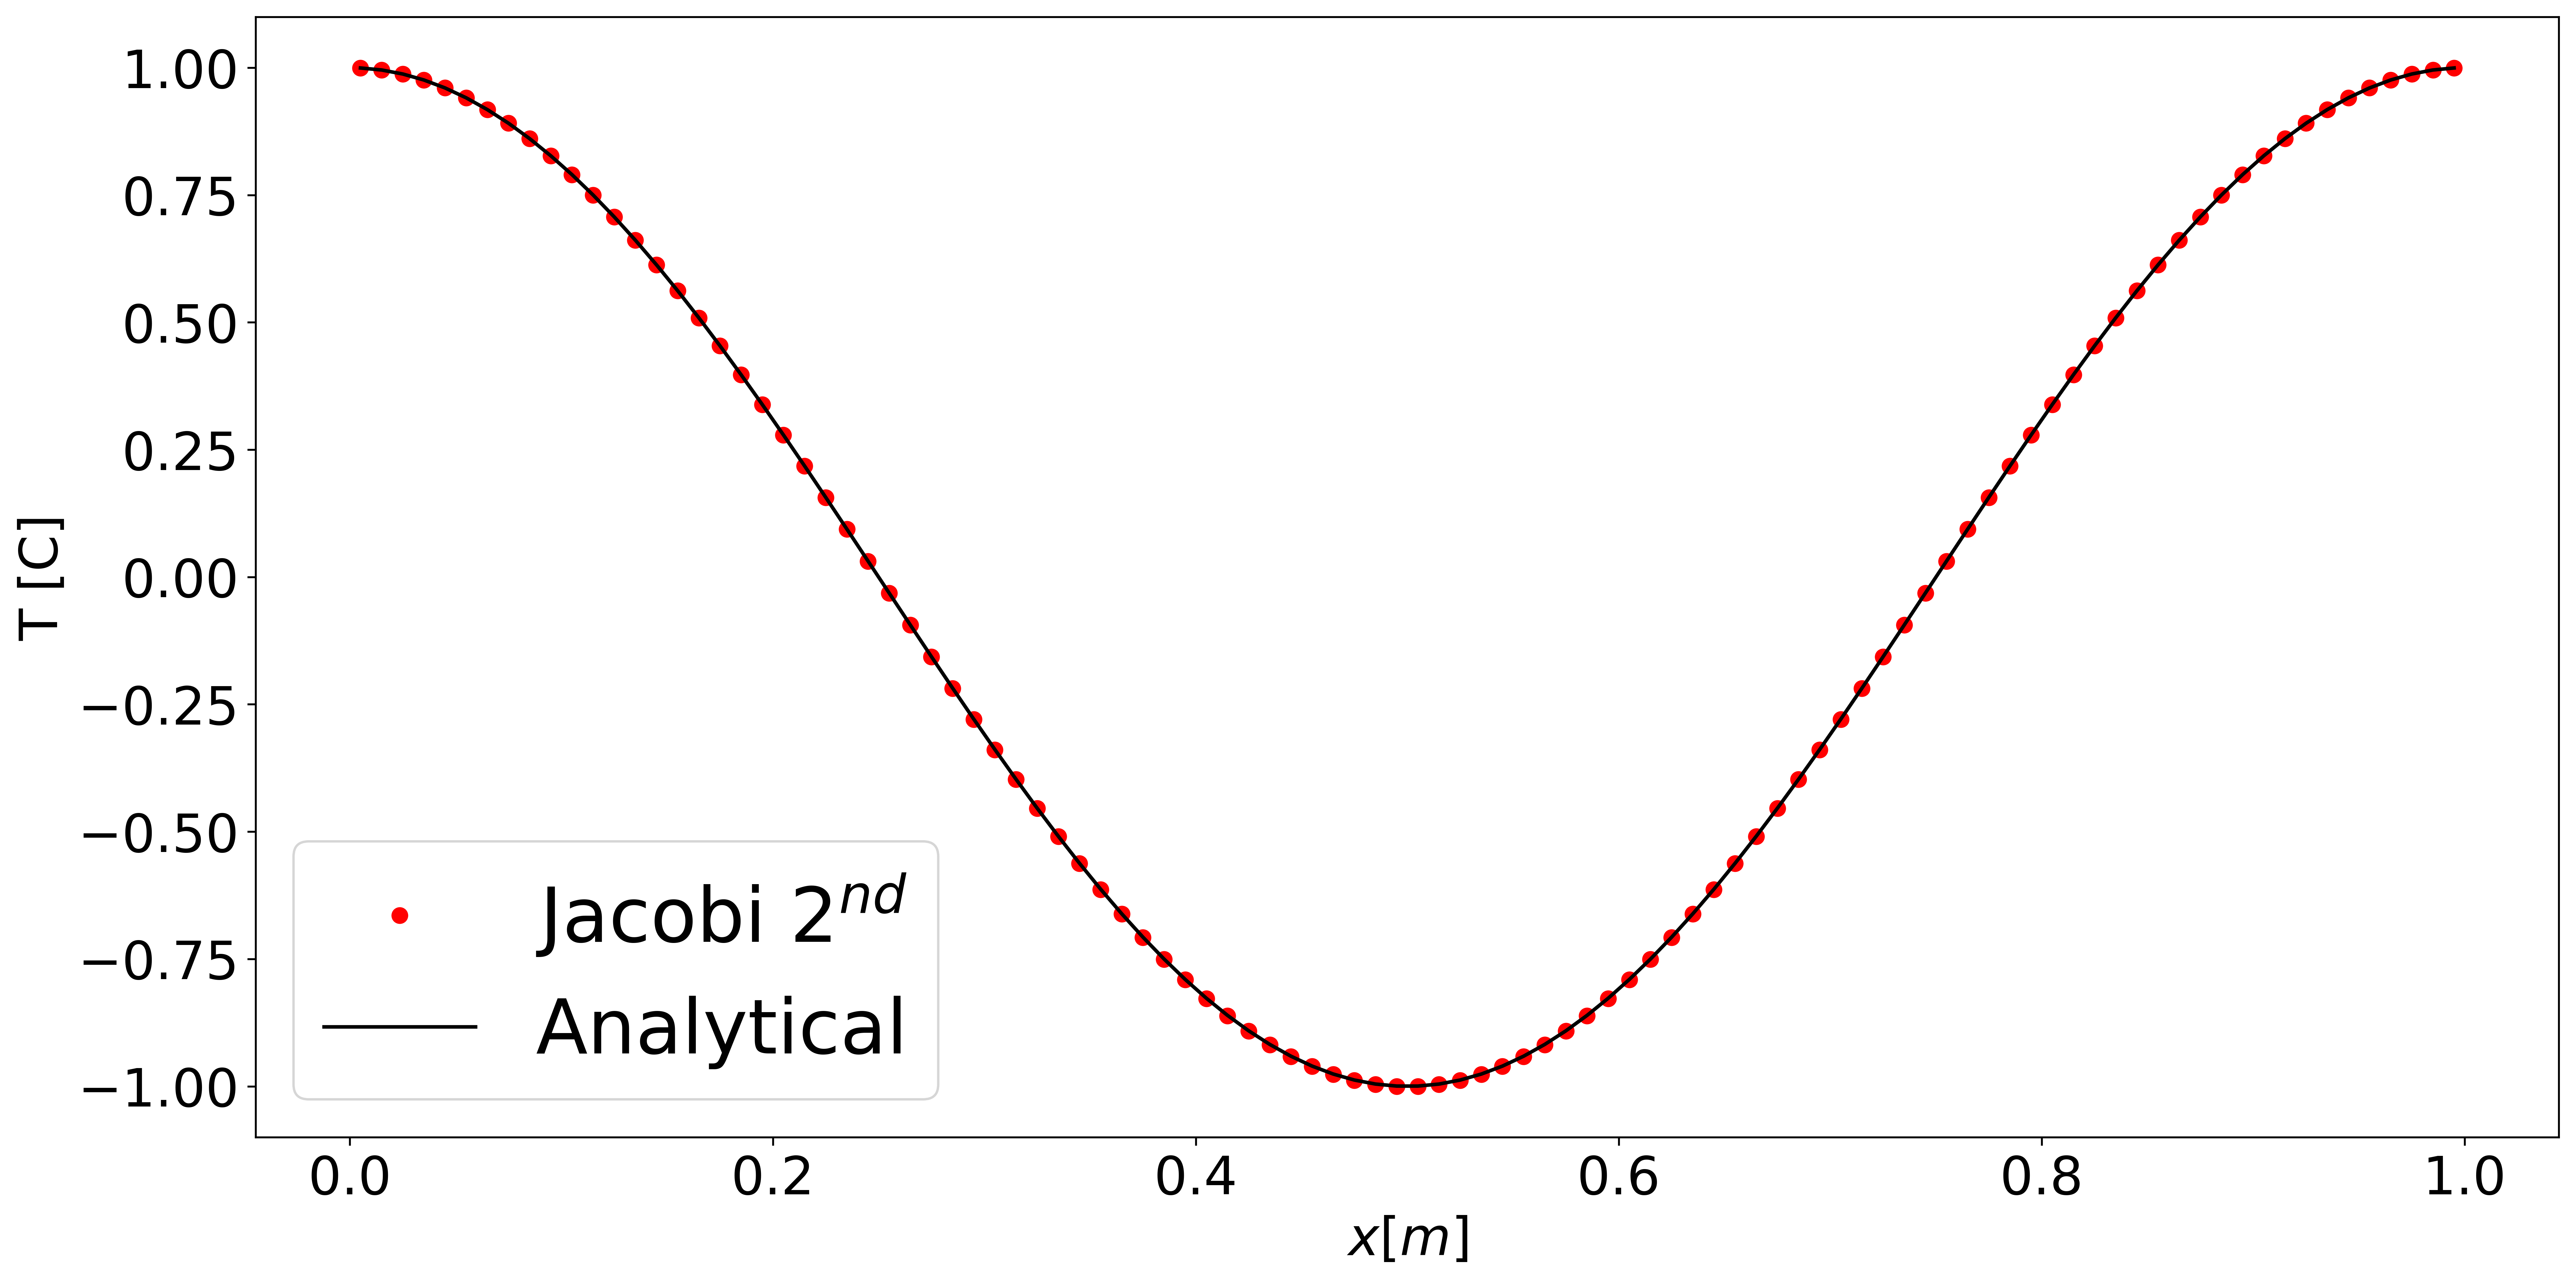
\includegraphics[width=\linewidth,keepaspectratio, trim = 0cm 0cm 0cm 0cm,clip]{Project1photos/plot_Jacobi_1D_order2_n100.png}
\end{minipage}
\begin{minipage}[]{\linewidth}
%\vspace{-15mm}
  \centering
    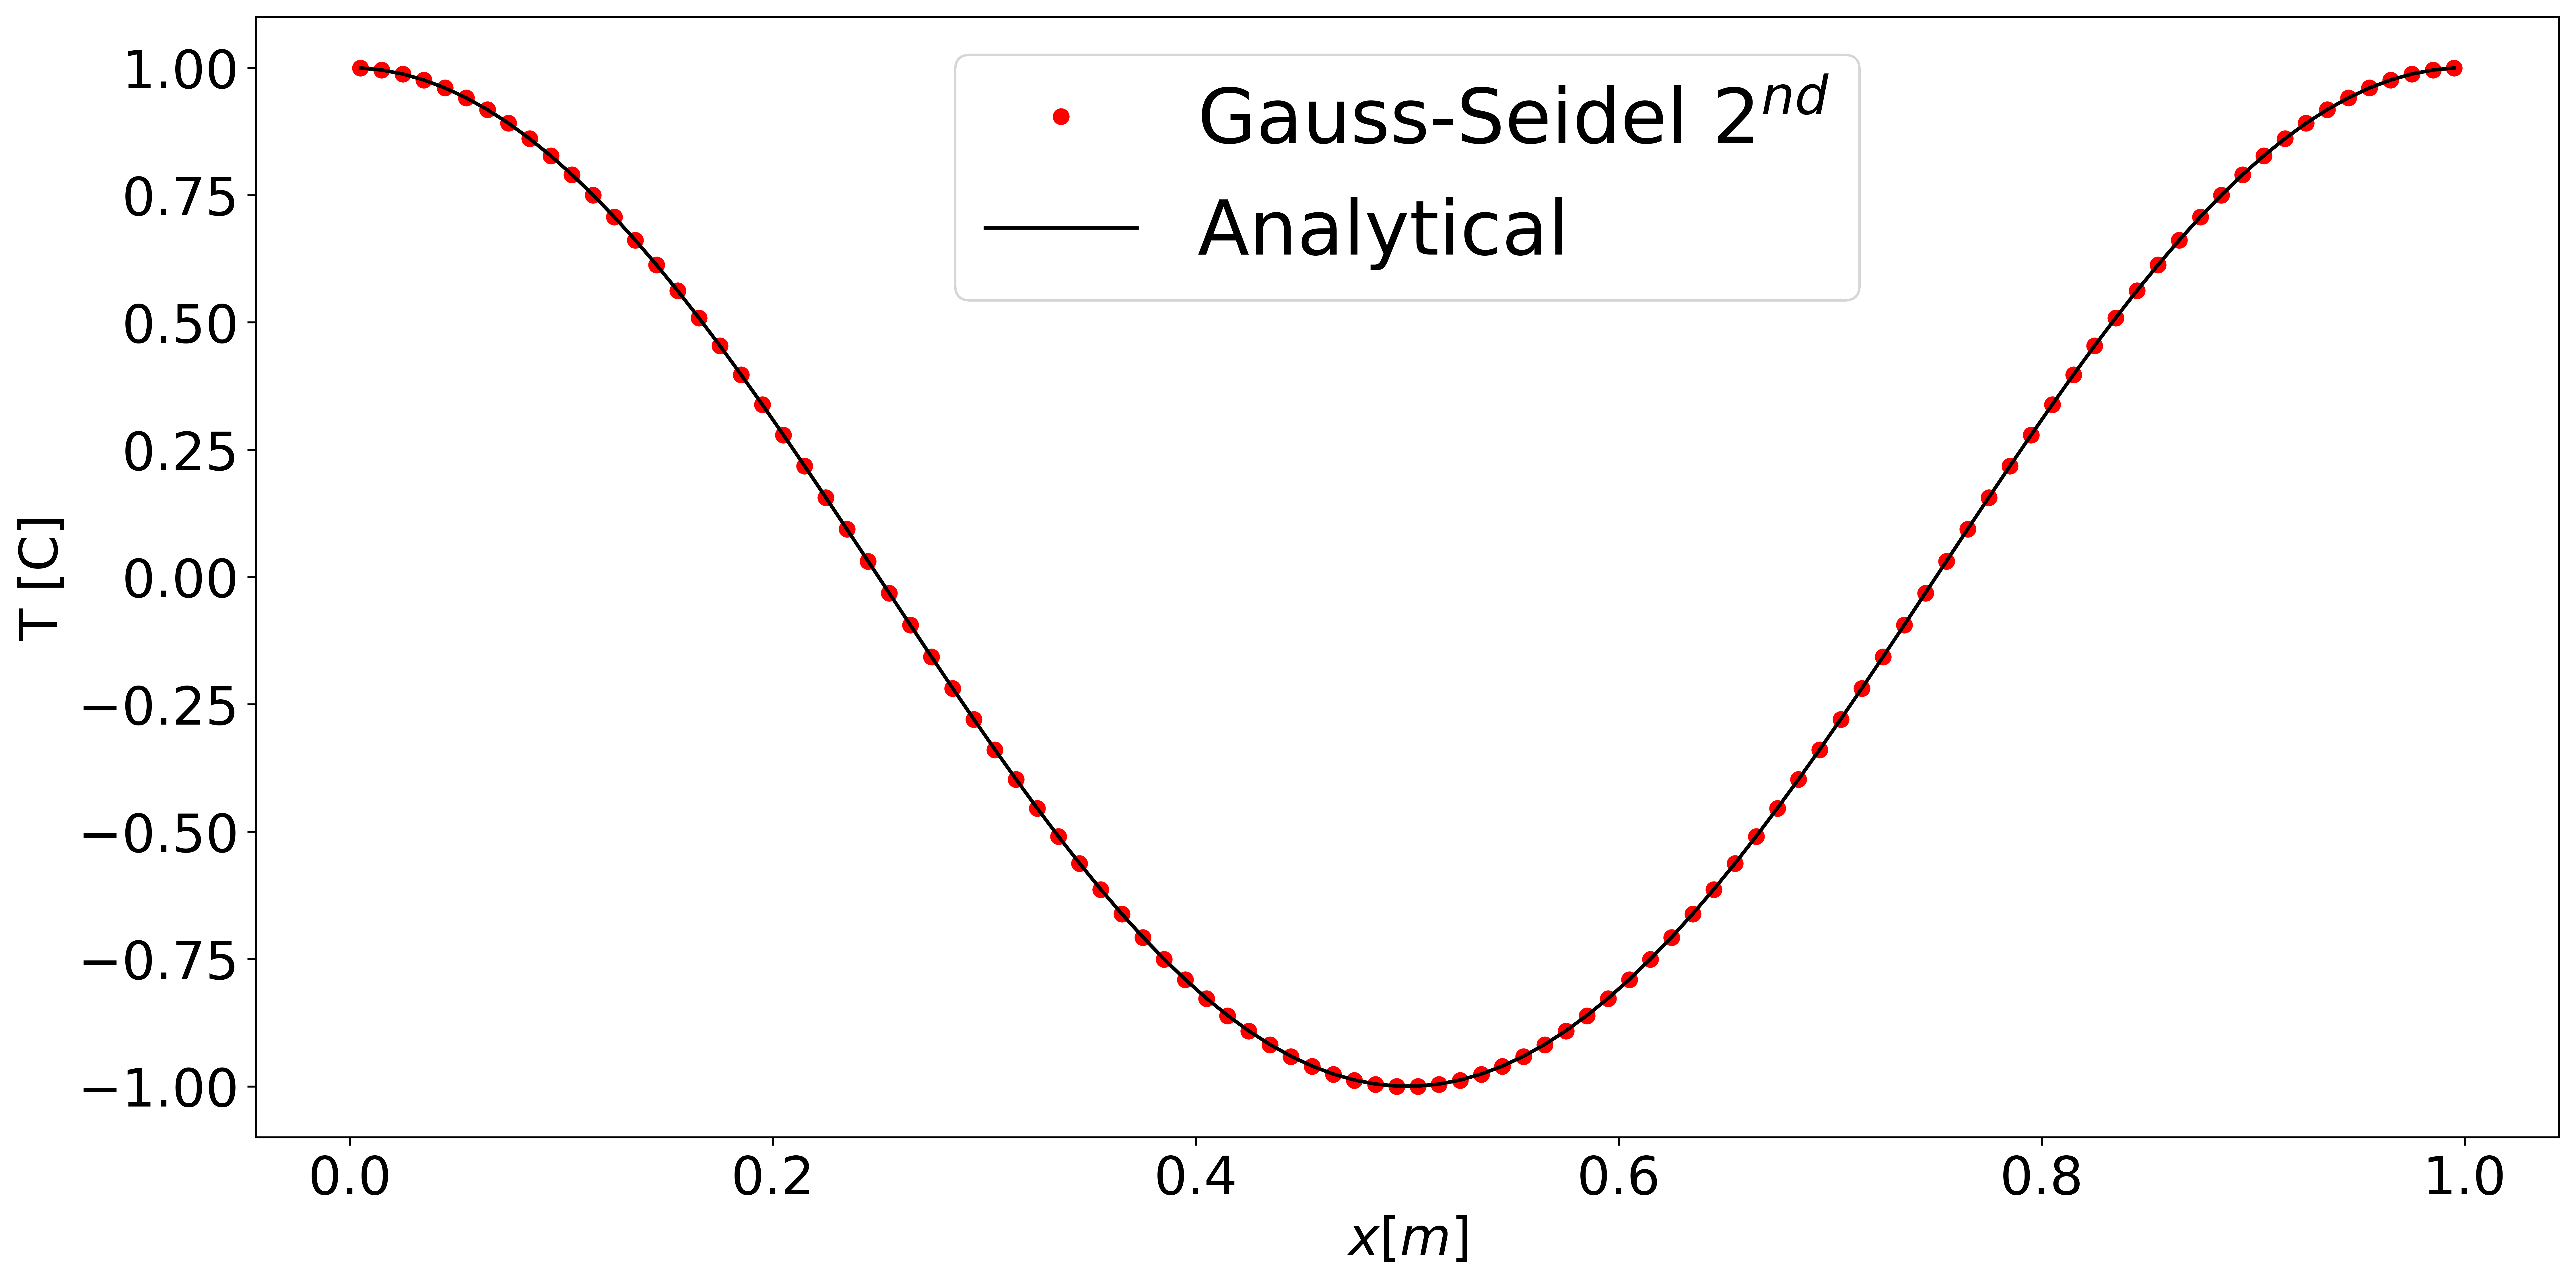
\includegraphics[width=\linewidth,keepaspectratio]{Project1photos/plot_GS_1D_order2_n100.png}
\end{minipage}
\caption{Results for the case of 1D tests, second order finite differencing, $N=100$ using Jacobi (top) and Gauss-Seidel (bottom) iterative solvers.} \label{fig:plot1D}
\end{figure}

\begin{figure}[htbp!] 
\begin{minipage}[htbp!]{\linewidth}
%\vspace{-15mm}
  \centering
    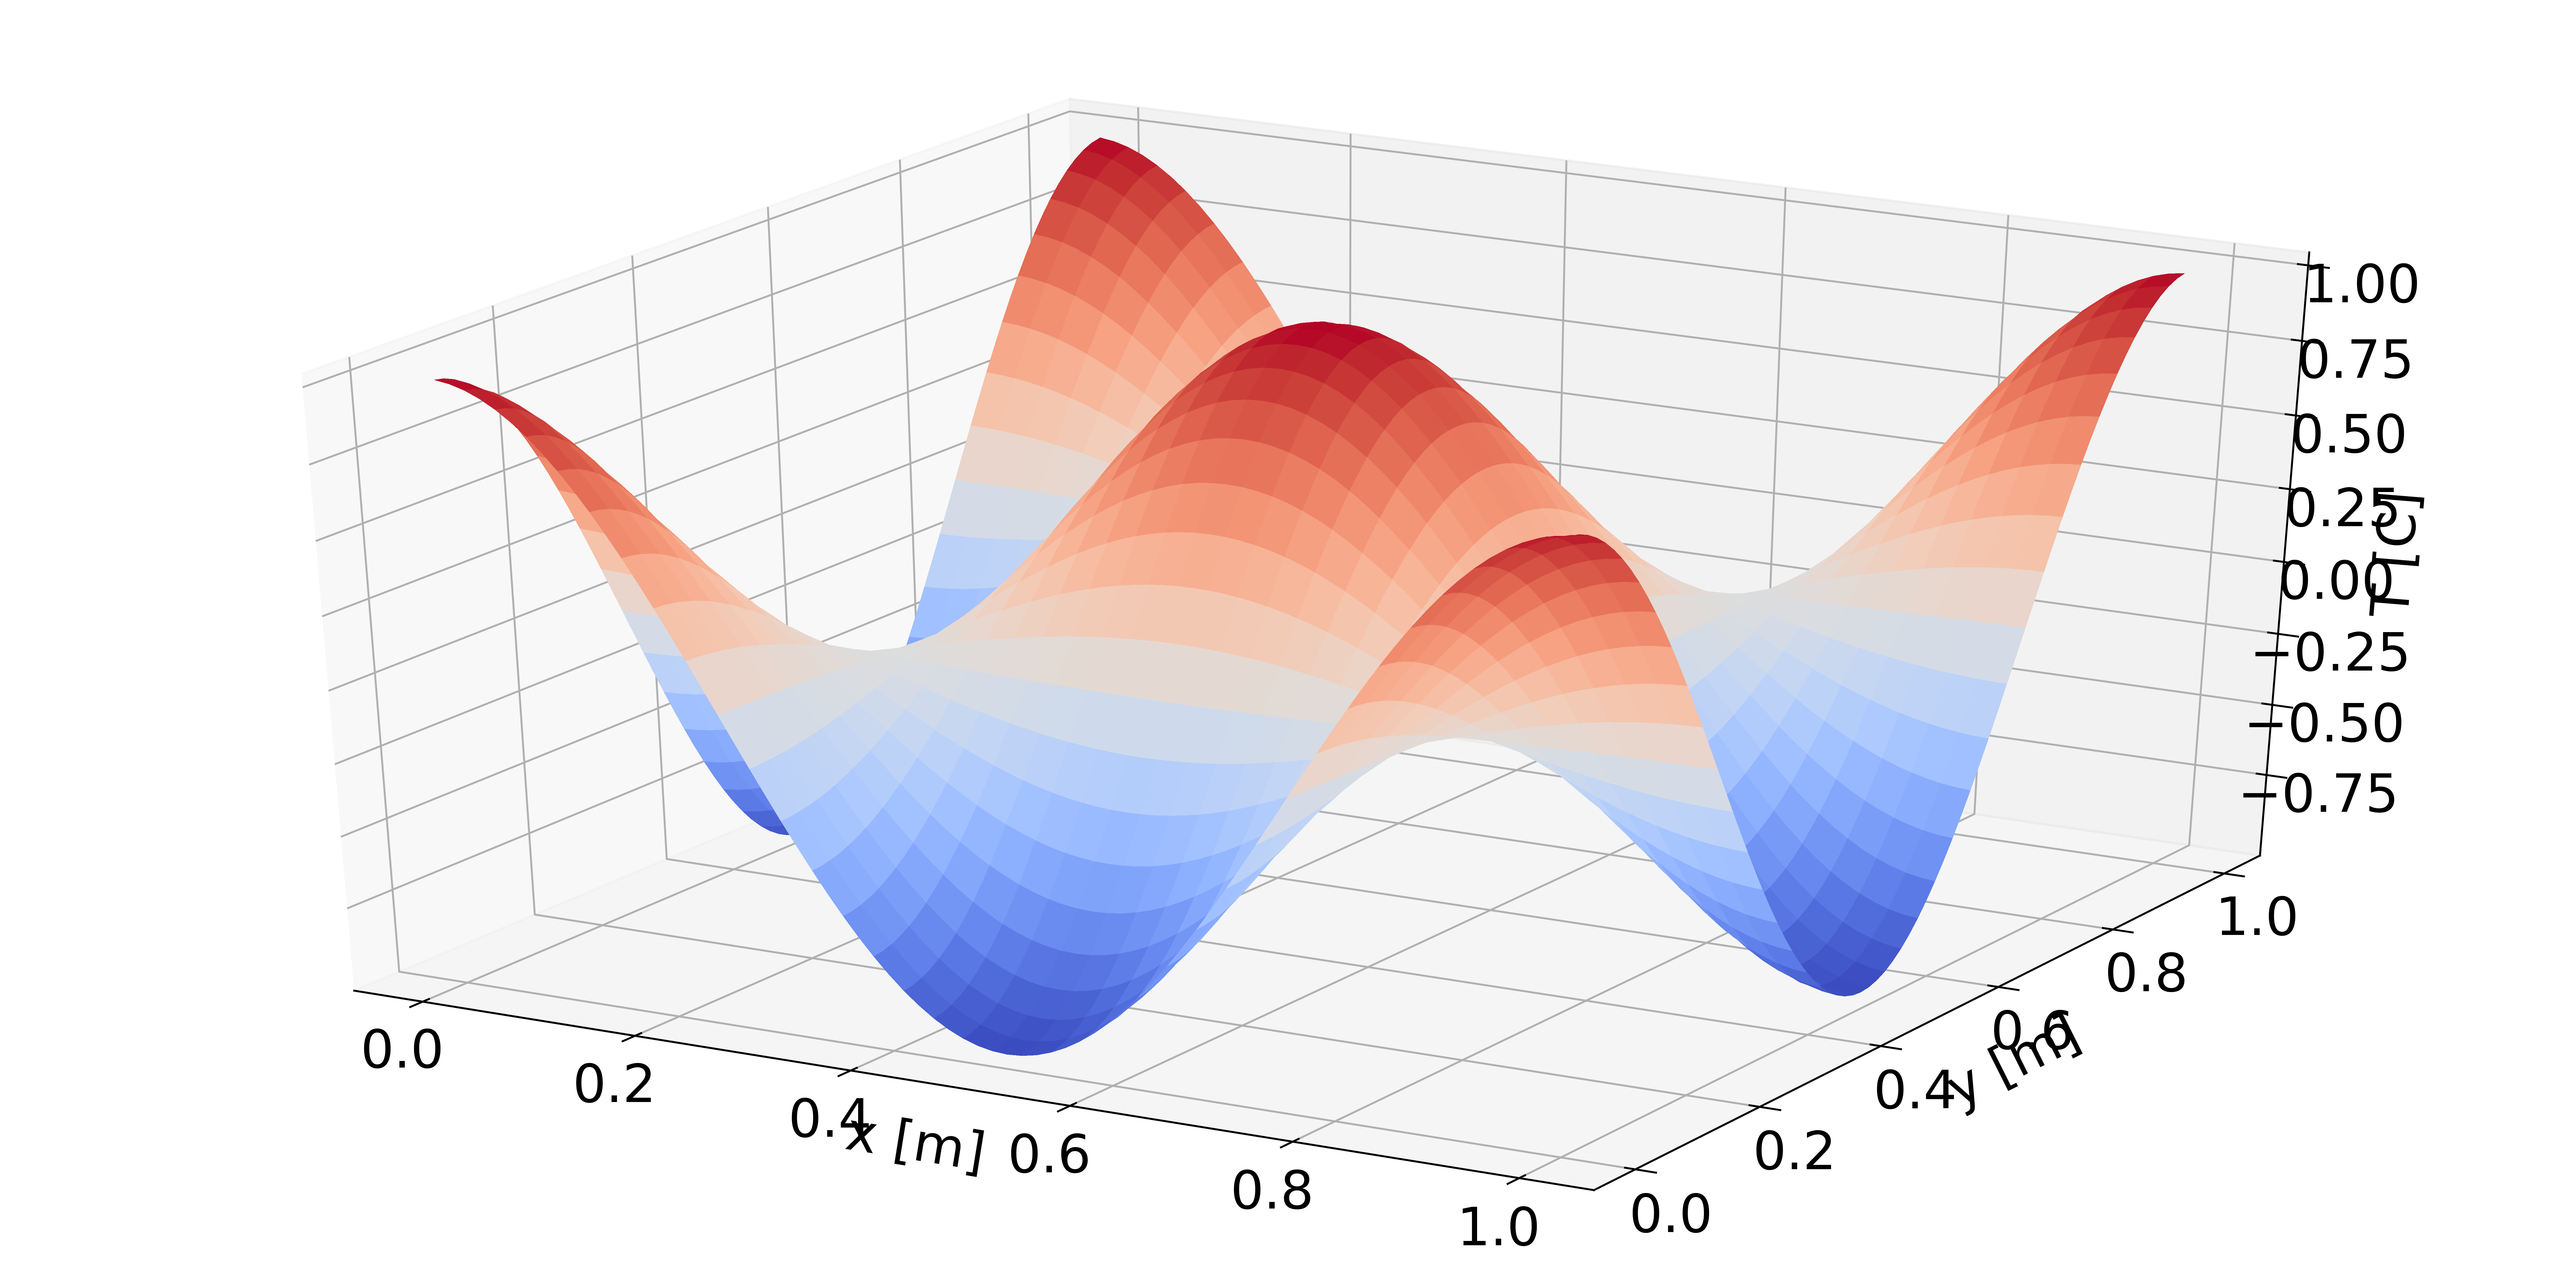
\includegraphics[width=\linewidth,keepaspectratio, trim = 0cm 0cm 0cm 0cm,clip]{Project1photos/plot_Jacobi_2D_order2_n75.png}
\end{minipage}
\begin{minipage}[htbp!]{\linewidth}
%\vspace{-15mm}
  \centering
    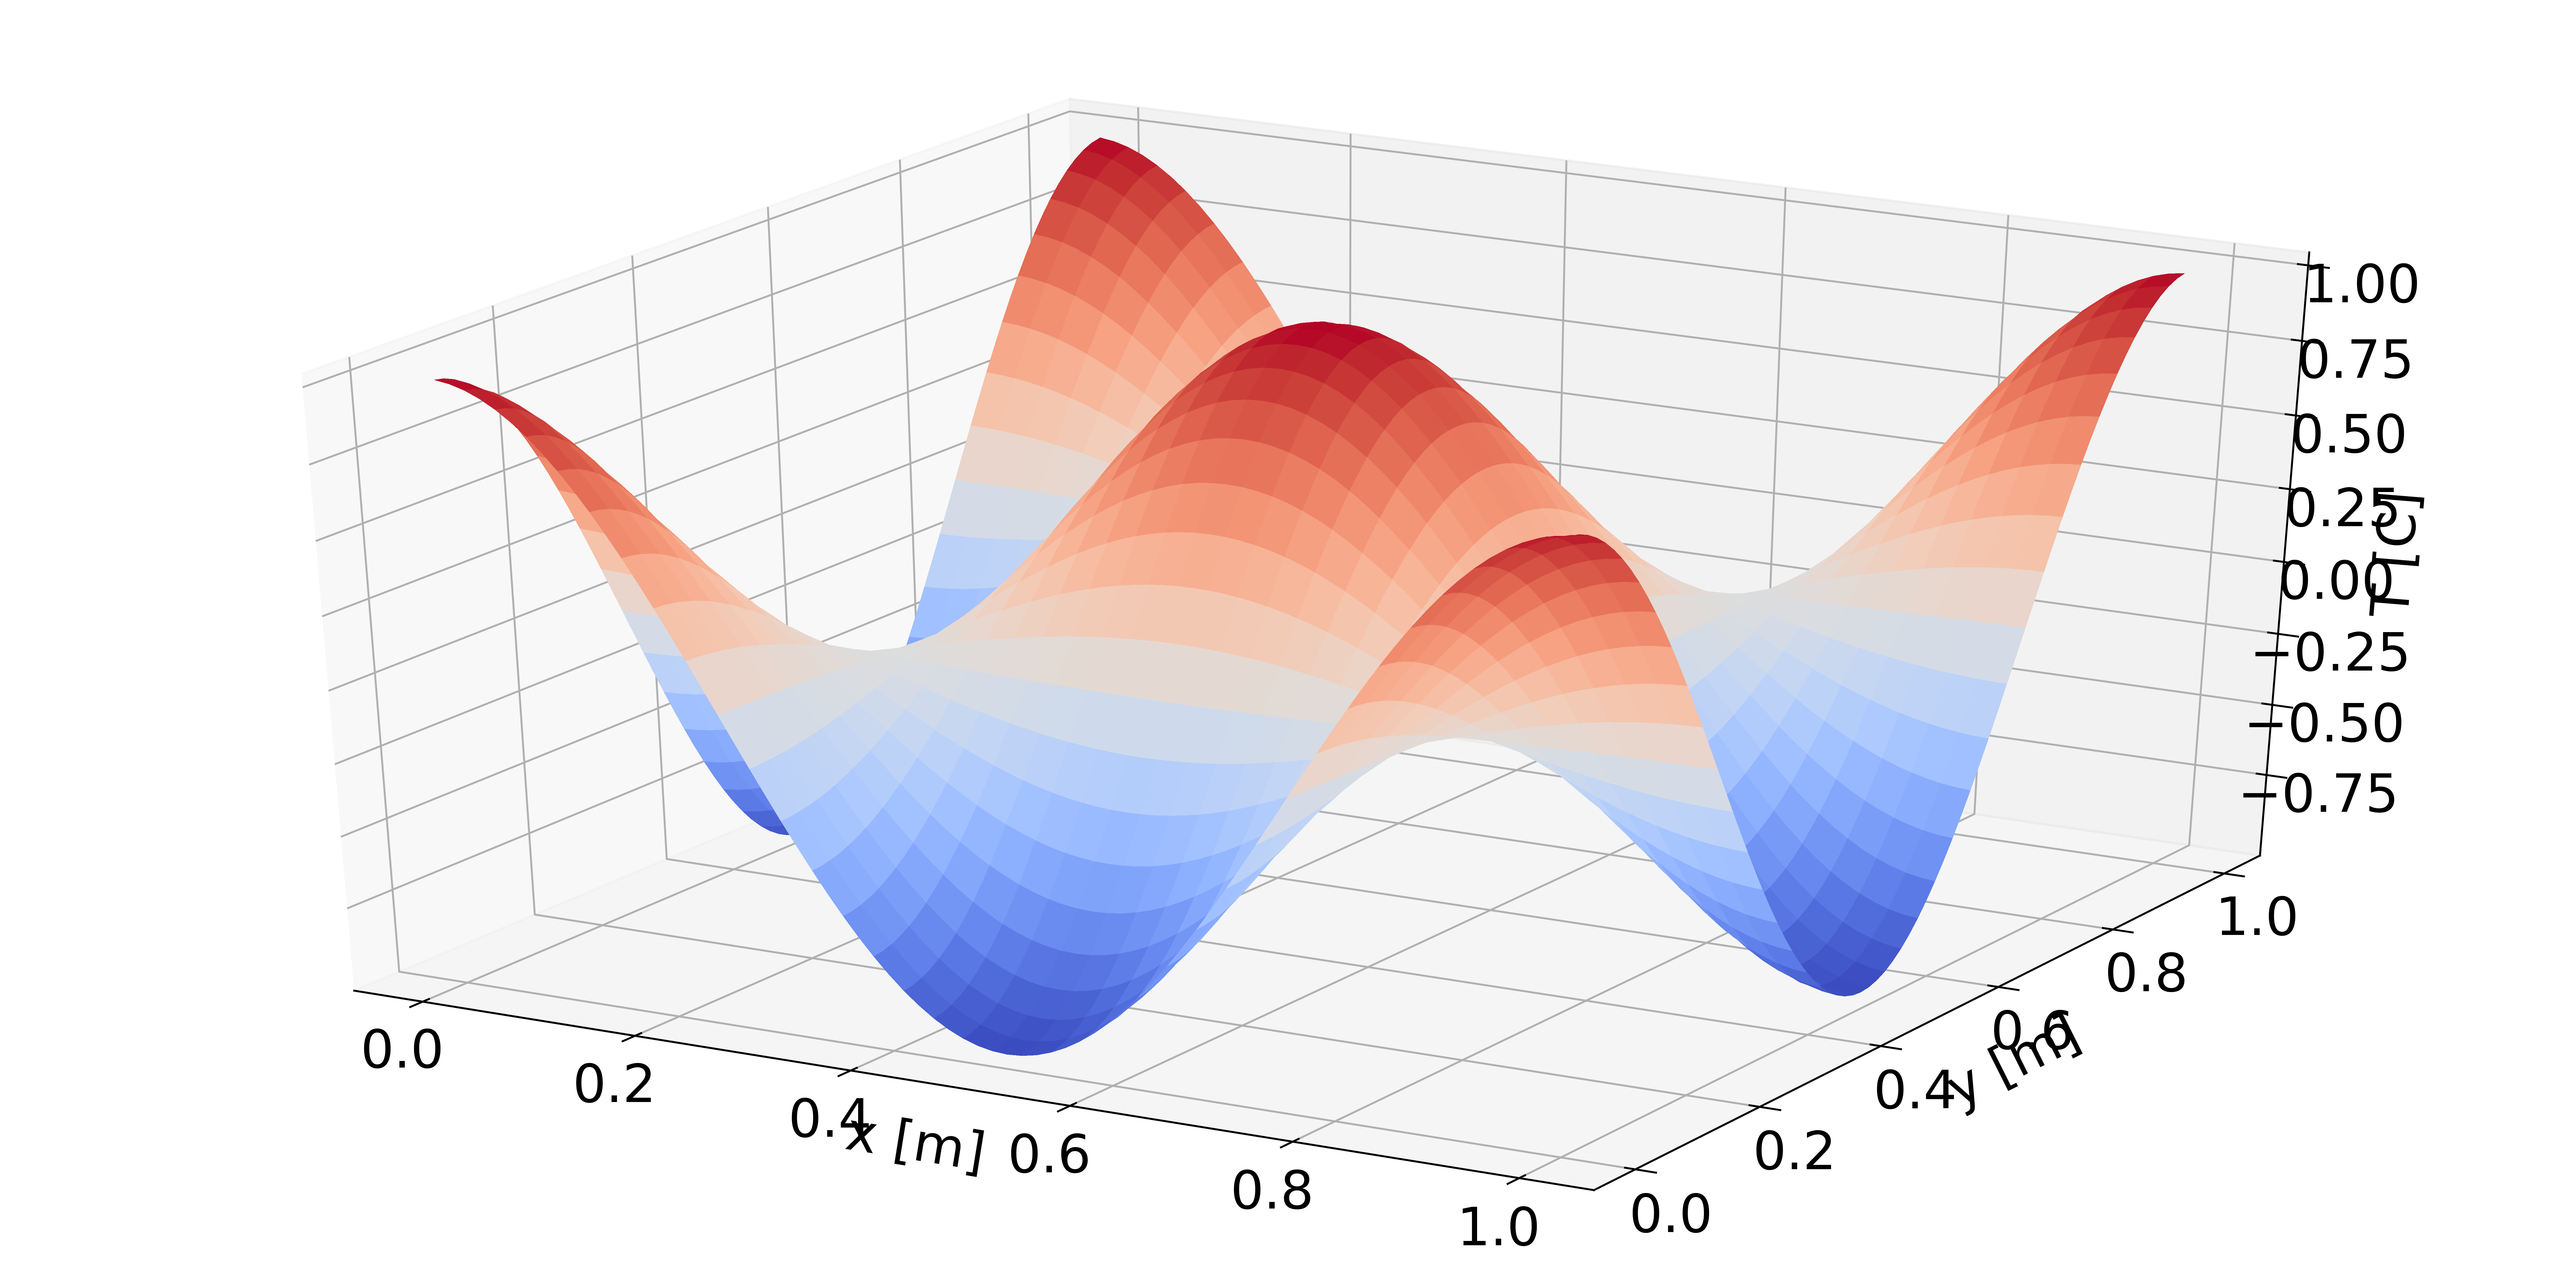
\includegraphics[width=\linewidth,keepaspectratio]{Project1photos/plot_GS_2D_order2_n75.png}
\end{minipage}
\begin{minipage}[htbp!]{\linewidth}
%\vspace{-15mm}
  \centering
    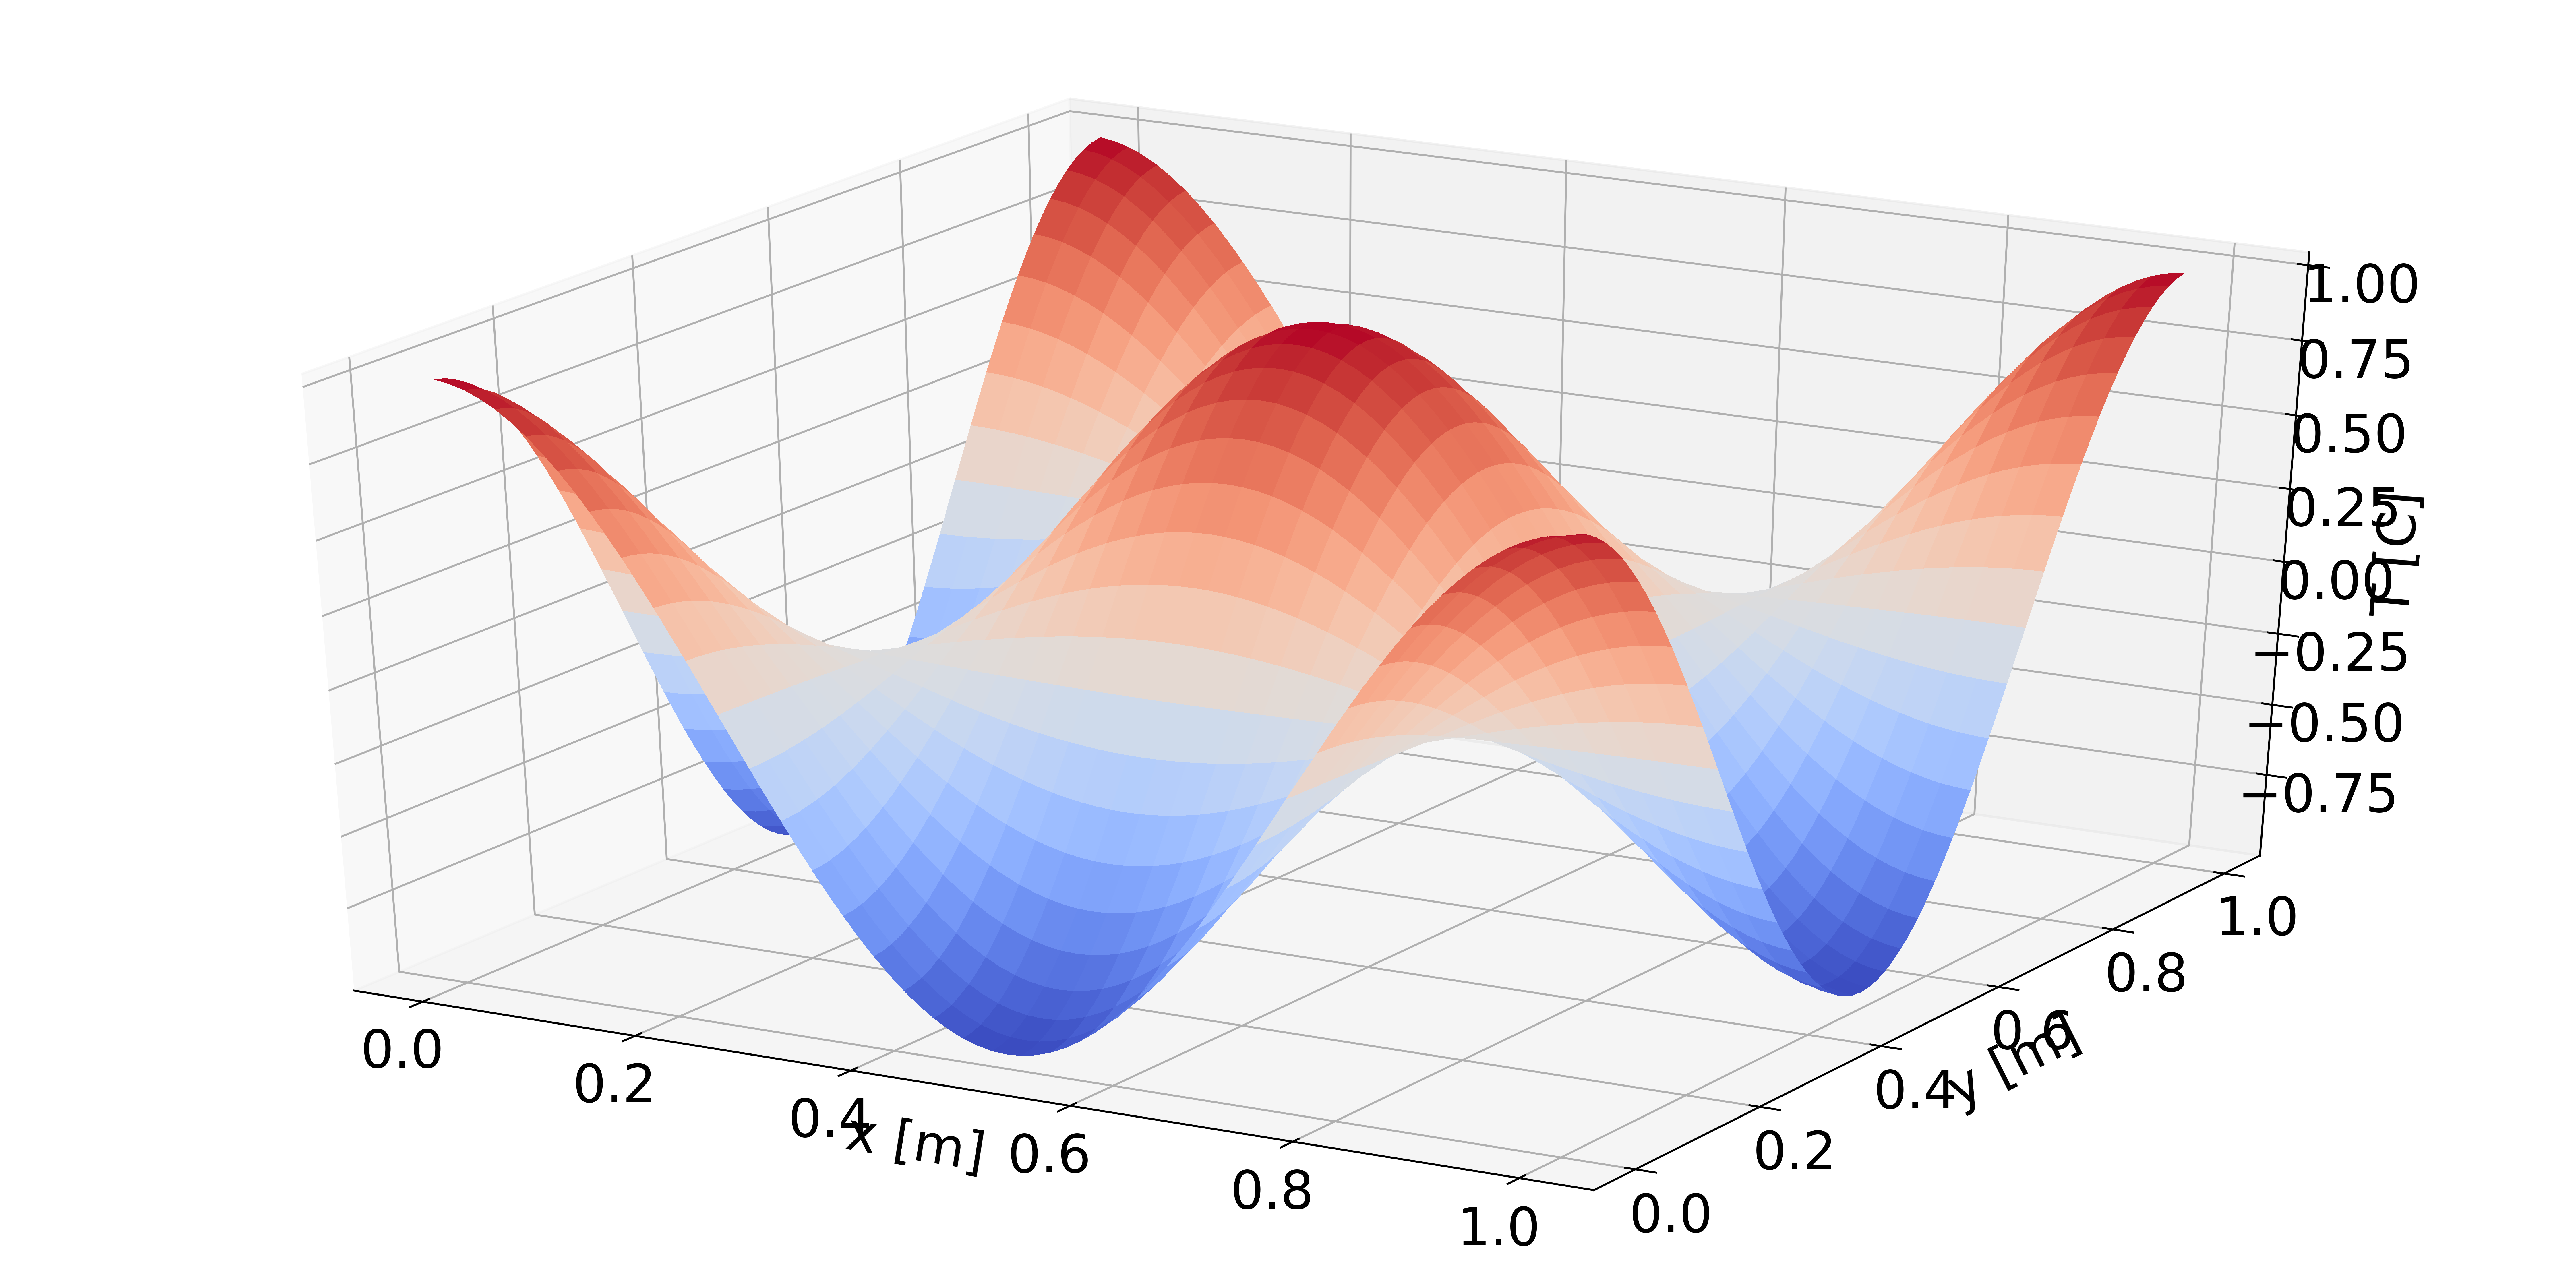
\includegraphics[width=\linewidth,keepaspectratio]{Project1photos/plot_Jacobi_2D_order2_n75_Analytical.png}
\end{minipage}
\caption{Results for the case of 2D tests, second order finite differencing, $N=75 \times 75$ using Jacobi (top), Gauss-Seidel (middle) iterative solvers and the bottom one is the analytical result.} \label{fig:plot2D}
\end{figure}



\newpage

\bibliographystyle{plain}
\bibliography{references}



%\section*{Appendix}
%Appendices are useful for putting in code or data.

\end{document}
